\chapter[Methodiken und Visualisierung]{Methodiken und Visualisierung für Continuous-Integration und Feature-Branches}
\label{ch:visu_meth}

Im vorangegangenen Kapitel wurde dargelegt, was Continuous-Integration und Feature-Branches sind und wie diese Techniken in der Softwareentwicklung angewendet werden. Zudem wird darauf eingegangen, welche Schwierigkeiten mit der Verwendung dieser Techniken einhergehen und dementsprechend Lösungen erfordern. 
Die nachfolgenden Abschnitte sollen mögliche Methodiken und Visualisierungen beleuchten und dadurch Lösungsansätze anbieten. Es wird auf Schwierigkeiten von bekannten Techniken und Methodiken eingegangen und erläutert, wie häufige Probleme vermieden werden können.

\section{Continuous-Integration und Feature-Branches}

Continuous-Integration und Feature-Branches sind beides Techniken, um die Kollaboration zwischen Entwicklern zu fördern. Continuous-Integration fordert die Integration in den existierenden Codestand für jede Änderung. Durch die Verwendung des Trunk-Based-Developments, ist das gesamte Team von dieser Integration direkt betroffen. Ist die Integration fehlerhaft, wird somit für die Dauer der Behebung das gesamte Team angehalten, bei der Behebung zu helfen. Der Feature-Branch-Ansatz hingegen lässt Änderungen ohne Integration parallel existieren. Folgt man der Gitflow-Verwendung von Feature-Branches aus Kapitel~\ref{subsec:gitflow}, wird auch hier eine Integration gefordert. Allerdings erst deutlich verzögert, etwa zu einem Release. Feature-Branches bieten somit einen Integrationsvorgang, ohne das Team zu blockieren. Allerdings wird der Zeitpunkt der Integration verzögert. In dieser Zeitspanne können weitere Änderungen hinzukommen. Jeder dieser Änderungen muss wiederum auf den Release-Branch integriert werden. Damit steigt der Aufwand sukzessive, über die Lebensdauer des Feature-Branches. Im ungünstigsten Fall eskaliert dieser Vorgang in einem \glqq big scary merge\grqq{} oder \glqq big bang merge\grqq{}, wie in Kapitel~\ref{sec:feature-branches} beschrieben. Dieses Risiko sollte gemindert werden, durch eine regelmäßige und kontinuierliche Integration mit dem Integrations-Branch.\\

\blockquote {Continuously is more often than you think.}\footcite[vgl.][Kap. Continuous Integration]{humble2010}\\

Besonders aufwändige Arbeiten sollten stets in kleinere Arbeitspakete gegliedert werden. Dies ermöglicht teilweise eine fokussierte Abarbeitung und Parallelisierung der Arbeiten. Bestimmte Arbeitsschritte werden aufwändiger, umso länger sie nicht bearbeitet werden. Bei solchen Tätigkeiten ist eine zeitnahe Bearbeitung zu priorisieren.
Angewendet auf die Integration von Feature-Branches sollten diese regelmäßig den Basis-Branch integrieren. Die erhöhte Frequenz vereinfacht die einzelnen Integrationsschritte.\\

\blockquote {When it is painful, the way to reduce the pain is to do it more frequently, not less}\footcite[vgl.][S.24]{humble2010}\\

Viele einzelne Integrationsschritte helfen die einzelnen Änderungen und ihre Motivation leichter zu erkennen. Dadurch sind komplizierte Merges leichter durchzuführen und es entstehen weniger Folgefehler.
 
Zielstellung der Vereinigung von Continuous-Integration und Feature-Branches ist folglich eine kontinuierliche Integration ohne Blockaden für andere Entwickler. Es muss definiert werden, wie Entwicklungssysteme und -werkzeuge ineinander greifen und es sollten Regeln und Strukturen definiert werden, um einen Ablauf mit nur wenig Reibungspunkten zu gewährleisten.

\subsection{Automatisierter Test von Feature-Branches}

Als erster Schritt zur Verschmelzung von Continuous-Integration und Feature-Branches ist es notwendig, jede Änderung automatisch zu testen. Dazu muss jede Änderung auf einem Feature-Branch in einem zentralen Repository bereitgestellt werden. Der Stand des Feature-Branches sollte wie in Kapitel~\ref{sec:automation-software} \nameref{sec:automation-software} beschrieben, erstellt und getestet werden.

Prinzipiell besteht die Möglichkeit, einen Test der Änderungen manuell auf dem Entwicklersystem auszuführen. Dieses Vorgehen erfordert allerdings eine hohe Anzahl an Werkzeugen und blockiert den Entwickler für diesen Zeitraum.

Die Bereitstellung in einem zentralen Repository ermöglicht es, statische und syntaktische Analysen zu erstellen. Die Ausführung der vollständigen Test-Suite erlaubt semantische Analysen. Die zentrale Aufbereitung der Ergebnisse der Analysen ermöglicht es allen Projektteilnehmern, eine Einschätzung des Feature-Branches vorzunehmen.

\subsection{Bewertung von Änderungen - Software-Metriken}
\label{subsec:main-metrics}

Tom DeMarco schrieb über Software-Metriken\footcite{demarco1986}:

\blockquote{You can’t manage what you can’t control, and you can’t control what you
don’t measure. To be effective software engineers or software managers, we
must be able to control software development practice. If we don’t measure
it, however, we will never have that control.}

Um Änderungen an einer Softwareanwendung zu bewerten und automatisiert Entscheidungen zu treffen, müssen die Änderungen quantifiziert und mit Vergleichswerten in Beziehung gesetzt werden. Für die Quantifizierung können Software-Metriken aus  Kapitel~\ref{subsubsec:base-metrics} verwendet werden. Da Aussagen über Programmkomplexität und Umfang kein hinreichende Bewertung ermöglichen, müssen zudem Verfahren zur Verifikation herangezogen werden. Die übliche Variante hierfür, ist eine umfangreiche Test-Suite und je nach Anwendung auch Verfahren, wie die in Kapitel~\ref{subsubsec:base-verification} beschriebene Modellprüfung und die abstrakte Interpretation.

In der Praxis werden automatisiert oft nur Tests verwendet. Der geringer Aufwand für ihre Erstellung und eine gute Skalierbarkeit sorgen für einen flexiblen Einsatz. 

Einzelne Ergebnisse durch Metriken können nicht für die Bewertung eines automatischen Software-Builds verwendet werden. Die Abbildung auf eine einheitliche Skala oder der Vergleich mit Fixpunkten erlaubt eine Bewertung der Ergebnisse. Die Auswahl der Fixpunkte ist stark abhängig von der verwendeten Metrik. Komplexitäts-, Umfangs- und Strukturmetriken liefern Werte, die nur schwer automatisiert zu bewerten sind. Hier bietet sich die Betrachtung der kurz- und langfristigen Änderung an. Sprunghafte Änderungen sollten dabei von besonderer Signifikanz sein. Prüfungen auf den Grad der Erfüllung eines Aspektes sind gut zu automatisieren. 

Die Testabdeckung einer Softwareanwendung kann auf 80\% festgelegt werden und darf an keiner Stelle unterschritten werden. Eine solche Prüfung sollte einen direkten Einfluss, auf das Ergebnis des automatisierten Software-Builds ausüben. Wird die Testabdeckung von 80\% angestrebt, kann dieser Zielwert auch schrittweise erreicht werden. Angefangen auf dem Wert der aktuellen Testabdeckung, wieder dieser Grenzwert schrittweise erhöht. Wird die Testabdeckung überschritten, passt sich der Grenzwert nach oben an. Auf diese Weise ist die Erhöhung möglich, allerdings nicht die Verringerung der Testabdeckung. Sinkt die Testabdeckung unter den neuen Grenzwert, schlägt der Software-Build fehl. Diese schrittweise Erhöhung ist ebenso für andere Grenzwerte denkbar.

Die Verwendung von Metriken und Testfällen erlauben keine grundsätzliche Aussage über die Qualität der Software. Richtig angewendet und gewartet erlauben sie eine zuverlässige Absicherung des automatischen Software-Builds.

\subsection{Automatisches Zusammenführen}

Das Zusammenführen von Änderungen ist ein schwieriges Unterfangen. Während der Merge von Codeständen häufig automatisch möglich ist, kann keine semantische Validierung während des Merges vorgenommen werden. Die Validierung kann erst nach dem Merge, durch die Ausführung einer Test-Suite erfolgen. Zusätzliche Informationen können durch die Ausführung von Metriken gewonnen werden.

\subsubsection{Fastforward-Merges}

Fastforward-Merge ist ein Fachbegriff, der in der Versionsverwaltung mit Git verwendet wird. Es bezieht sich auf das Verschieben eines Branch-Zeigers zu einem anderen Branch-Zeiger, ohne die Zusammenführung von Änderung. Es werden lediglich bestehende Änderung des abzweigenden Branches auf den Basis-Branch übertragen.
Fastforward-Merges sind gut zu automatisieren, da sie komplett ohne manuellen Eingriff von Git durchgeführt werden können. Dadurch können verschiedene automatisierte Verfahren auf Basis eines Fastforward-Merges aufgebaut werden.

Es ist eine gängiges Verfahren nur Fastforward-Merges zu erlauben. Dadurch wird die Verantwortung eines potentiellen Merge-Konfliktes immer zum Autor der Änderung delegiert.
In der Strategie \glqq Read-Only-Master-Branch\grqq{}\footcite{master-read-only} wird dies deutlich. Ziel der Methodik ist es Änderungen durch einen Merge immer vollautomatisch auf einen Integrations-Branch überführen zu können. Die Garantie keinen Merge-Konflikt zu erhalten, ist nur bei einem Fastforward-Merge gegeben. Ist diese Voraussetzung geschaffen, kann allen Entwicklern die Rechte entzogen werden auf dem Master-Branch zu veröffentlichen. Dadurch sind sie gezwungen auf den automatisierten Merge zurückzugreifen. Der automatisierten Vorgang ist nur die einzige Möglichkeit Änderungen zu veröffentlichen und kann als Aufhänger für zahlreiche automatisierte Qualitätssicherungsmaßnahmen genutzt werden. Üblicherweise sollte die Ausführung bestehende Test-Suits eine der Qualitätsmaßnahmen sein.

\subsubsection{Flüchtige Release-Branches}
\label{temporary-releases}

Ein Release-Branch ist die Basis für alle release-fähigen Feature-Branches. Nachd der Erstellung des Release-Branches, werden schrittweise alle Feature-Branches, durch einen Merge auf den Release-Branch zusammengeführt. Ist der Vorgang abgeschlossen, wird der letzte Commit des Release-Branches mit einem Tag markiert. Der Release-Branch und alle Feature-Branches können theoretisch ab diesem Moment gelöscht werden. Der Release-Tag kann auf ein beliebiges System ausgeliefert werden.

Dieses Vorgehen kann zu Problemen führen, wenn Änderungen eines Feature-Branches wieder aus dem Release-Branch entfernt werden müssen. Zudem treten mögliche Merge\hyp{}Fehler und \hyp{}Probleme erst beim Zusammenführen mit dem Release-Branch auf.

Abhilfe könnte ein \glqq flüchtiger\grqq{}-Release-Branch schaffen. Dazu müssten alle Feature-Branches markiert werden, die für ein Release vorgesehen sind. Ein automatisierter Vorgang kann daraufhin alle markierten Feature-Branches auf ihre Kompatibilität prüfen. Alle kompatiblen Feature-Branches werden durch einen Merge auf einem Release-Branch zusammengefasst. Feature-Branches sind dann kompatibel, wenn sie sich ohne Merge-Konflikte auf den Release-Branch integrieren lassen. Das Ergebnis sollte nun von einem automatisierten Software-Build erstellt, validiert und gemessen werden. Ist der Software-Build erfolgreich, steht ein automatisch erstelltes Software-Inkrement. Dieses Software-Inkrement kann beliebig ausgeliefert werden. Schlägt der Software-Build fehl, existiert eine syntaktischer oder semantischer Fehler, der durch den Merge der Feature-Branches entstanden ist. Da der vollständige Vorgang automatisch abläuft, können Konflikte zwischen Feature-Branches frühzeitig erkannt und behoben werden. Im Gegensatz zu einem regulären Release-Branch, ist diese Variante nur flüchtig und wird vom System nach der Validierung und Messung wieder entfernt. Ein regulärer Release-Branch würde zahlreiche Merge-Commits enthalten und ließe sich durch die vielen Zwischenstände nur schwer für das Verfahren verwenden.

Ein Nachteil des Verfahrens ist die Auswahl der Feature-Branches. Die Reihenfolge mit der die Feature-Branches in einem Merge-Verfahren getestet werden, ist maßgeblich für die auftretenden Konflikte. Die Auswahl eines einzigen Feature-Branches ist möglich, wenn dieser mit allen weiteren im Konflikt steht. Sind alle anderen ohne Konflikt kombinierbar, wäre das möglicherweise eine schlechte Auswahl. Eine Auswahlstrategie ist daher ratsam, die Auswahl nach Priorität der Features wäre naheliegend.

Existierenden Konflikte zwischen Feature-Branches können durch einen Merge unter den Feature-Branches beseitigt werden. Dies führt zu einem weiteren Nachteil des Verfahrens. Werden Feature-Branches durch einen Merge kombiniert, können diese nicht mehr unabhängig entwickelt werden. Die kombinierten Feature-Branches werden dadurch in einem Continuous-Integration nahen zustanden überführt. Die Vorteile von Feature-Branches werden dadurch geschwächt.

Das Verfahren ist daher schlechter, wenn viele Konflikte unter den Feature-Branches auftreten. Existieren viele Abhängigkeiten innerhalb der entwickelten Softwareanwendung, steigt die Wahrscheinlichkeit für einen Merge-Konflikt. Somit ist die Effizienz des Verfahrens abhängig von der Kopplung der Komponenten in der Softwareanwendung.

In einem optimalen Szenario ist das Verfahren mit Continuous-Integration vergleichbar. Integrationskonflikte werden schnell erfasst und die Integration alle Arbeitsstände gefördert. Ob das Verfahren in der professionellen Softwareentwicklung effizient eingesetzt werden kann, ist nicht vorherzusehen.

\section{Automatisierte Erstellung von graphischen Übersichten}

Angesichts der Komplexität von Softwareanwendungen mit der Entwickler häufig konfrontiert sind, ist es essentiell die entscheidenden Informationen zusammenzutragen. Je nach Situation können dabei andere Ansichten und Übersichten wichtig sein. In stark gewachsenen Softwareprojekten können mit speziellen Visualisierungen Engpässe und interne Abgrenzungen gefunden werden. Es können Wachstum und Fortschritt eines Projektes visualisiert werden. Viele Ansichten erleichtern zudem die Kommunikation zwischen Projektteilnehmern. Technisch komplexe und schwer zu fassende Daten, können so leichter zugänglich gemacht werden.

Wesentlich bei diesen Ansichten ist der Aufwand für ihre Erstellung. Ansichten die einen hohen manuellen Aufwand erfordern, veralten schnell und werden nicht mehr genutzt. Im schlimmsten Fall liefern veraltet Ansichten falsche Informationen. Somit ist es entscheidend diese Ansichten und Übersichten automatisch zu erstellen. Über Metriken aus dem automatisierten Softwareerstellungsprozess, können die notwendigen Messwerte ermittelt werden. 

Da in graphische Übersichten Trends und Schwerpunkte erkannt werden sollen, bieten graphische Übersichten einen Vorteil gegenüber rein textbasierten Darstellungen. Ein einfacher und schneller Eindruck vom Projektfortschritt und der -Qualität kann damit erlangt werden.

Bewertungen von Feature-Branches und Releases können damit unterstützt werden.

\subsection{Übersicht zu Branches}

Szenarien, in denen viele Branches zum Einsatz kommen, müssen den dadurch entstehenden zusätzlichen Aufwand berücksichtigen. Werden die zahlreichen Zustände des Software-Codes nicht entsprechend behandelt, kann ein erhebliche Mehraufwand durch Aktualisierung und Merging der Branches entstehen. Somit ist es notwendig Branches schnell zu beurteilen und einordnen zu können.

Eine solche Übersicht müsste wichtigen Kriterien eines Branches gesammelt und übersichtlich bereit stellen. Solche Kriterien sind unter anderem:
\begin{itemize}
\item Alter des Branches,
\item beteiligte Autoren,
\item wie häufig in vergangener Zeit neue Änderungen auf den Branch eingebracht wurden (Puls) und
\item Kennzahlen des Branches zu Qualität und Fortschritt.
\end{itemize}

Durch diese Übersicht können schnell Entscheidungen getroffen werden, welche Branches in den Fokus der Entwicklung gerückt werden müssen. Alte oder bereits in den Codestand überführte Branches können gelöscht werden. Branches mit schlechten Kennzahlen können zu einem Refactoring eingeplant werden. 

\subsection{Übersicht zu Releases}

\begin{figure}[htbp]
  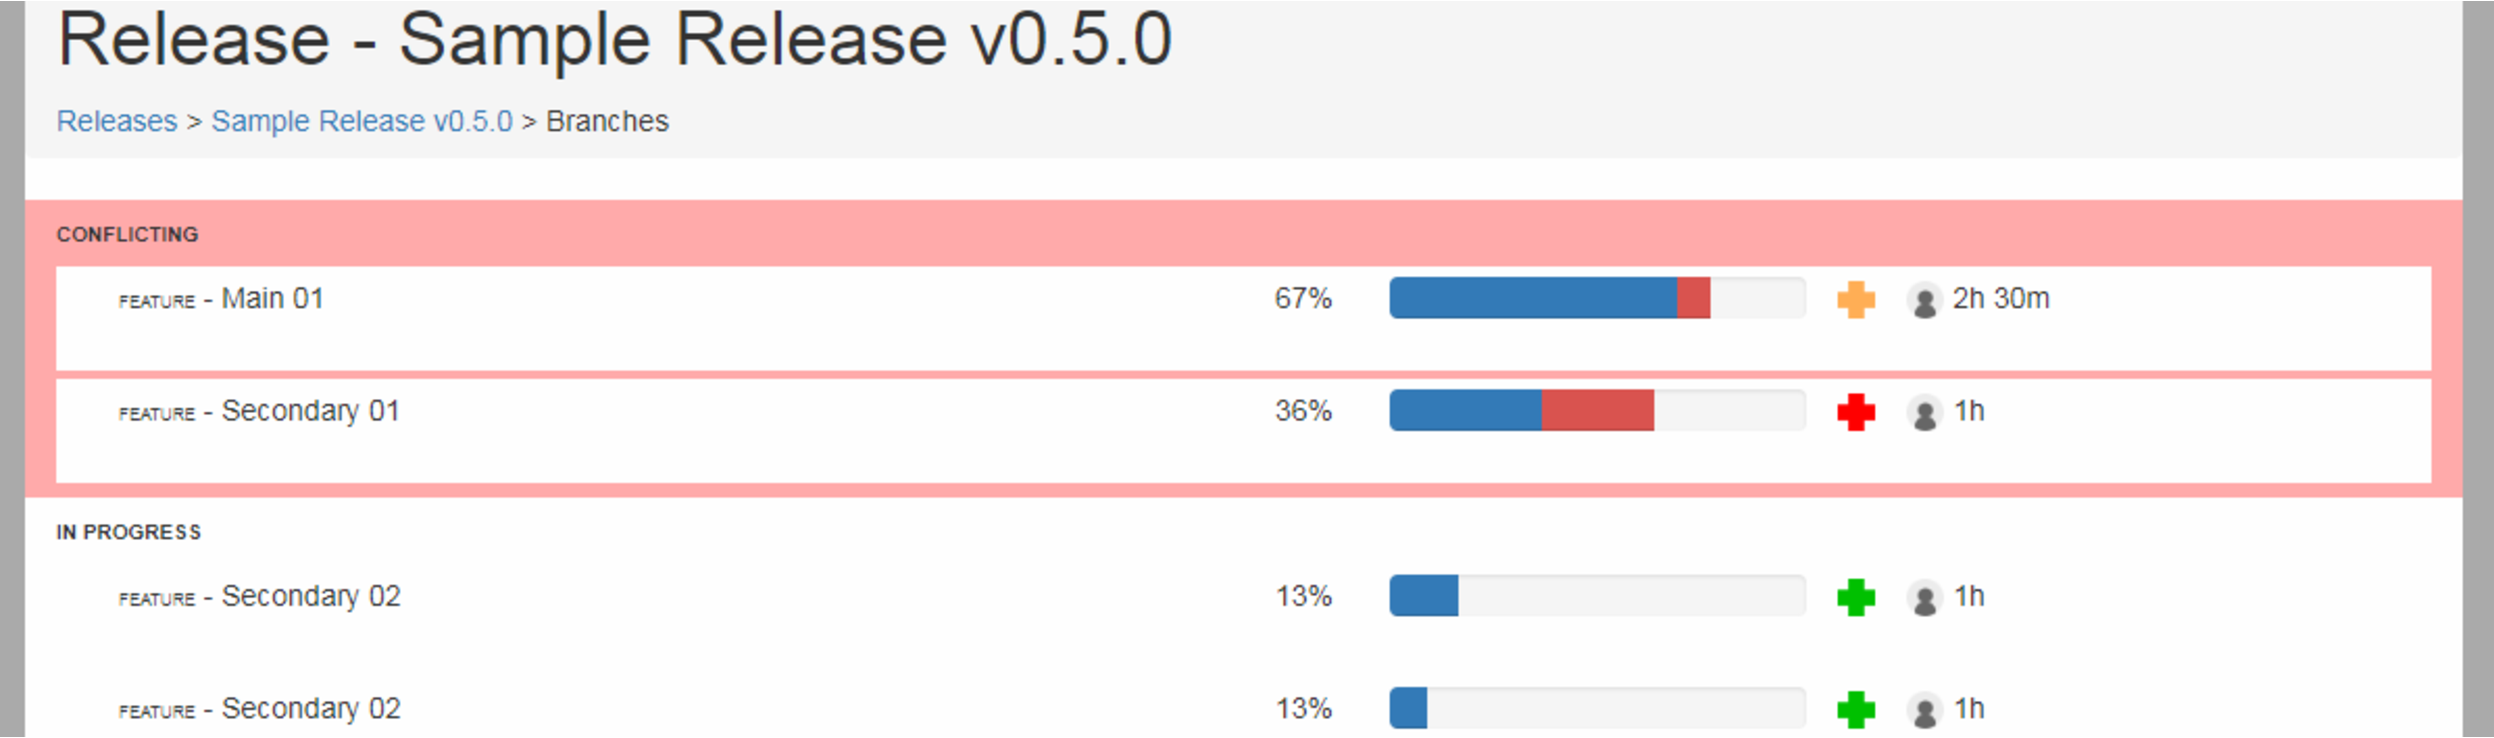
\includegraphics[
    width=\textwidth,
    height=\textheight,
    keepaspectratio
  ]{resources/release-branch_overview.pdf}
  \caption{Prototyp - Releaseübersicht}
  \label{prototype-release-overview}
\end{figure}

Angelehnt an die Branch-Übersicht und die angesprochenen \glqq flüchtigen\grqq{} Release-Branches, können auch Release-Ansichten bereit gestellt werden. Neben den bereits in der Branch-Übersicht erwähnten Kriterien, können weitere Kriterien visualisiert werden. Kriterien für das Zusammenspiel der für das Release geplanten Branches wären zum Beispiel:
\begin{itemize}
\item Konflikte zwischen Branches,
\item Abschätzung zum Fortschritt des Releases,
\item Branches mit geringem Fortschritt und
\item Blockierende Branches.
\end{itemize}

Die Visualisierung von Konflikten und Blockaden kann die Beurteilung eines Releases deutlich erleichtern. Die erleichterte Kommunikation von Konflikten hilft bei deren Fokussierung innerhalb eines Releases. Eine konkrete Aussage über den Fortschritt eines Releases ist nicht ohne Weiteres möglich. Es können allerdings Abschätzungen auf Basis des geschätzten Umfangs von Features vorgenommen werden. Zusammen mit Daten zu benötigter Arbeitszeit, getätigten Commits, Teststand und -abdeckung kann dieses Bild verbessert werden.

In Projekten verwendete Ticketverwaltungssysteme können eine ähnliche Ansicht bereitstellen. Diese beurteilen ebenfalls anhand von geplantem und gebuchtem Aufwand den Stand eines Releases.

Die zusätzlichen Informationen, aus dem Versionsverwaltungssystem, Tests und Metriken können die Release-Ansicht verfeinern. 

\subsection{Konfigurations- und Systemübersicht}
\label{subsubsec:configuration-system-overview}

Das Konfigurationsmanagement aus der automatisierten Softwareerstellung kann auch für eine System- und Konfigurationsübersicht verwendet werden. Zusammen mit Daten aus einer Systemüberwachung oder Virtualisierungs-Verwaltung lassen sich umfangreiche Rückschlüsse ziehen. 

Eine automatisierte Übersicht ist in verschiedenen Einsatzgebieten von Vorteil. Unabhängig davon ob eine voll automatisierte Virtualisierungs- und Container-Verwaltung eingesetzt wird oder ein manuelle administrierter Rechnerverbund.

In einer vollautomatisierten Virtualisierung werden Systeme automatisch bereitgestellt, verwaltet und wieder entfernt. Eine aussagekräftige Übersicht erleichtert sowohl die Fehlersuche als auch das Erstellen von Auswertungen zu den Systemen. Viele Virtualisierungs\hyp{}Verwaltungen sollten bereits zahlreiche Auswertungsmöglichkeiten bereitstellen. Aufgrund der allgemeingültigen Natur der Verwaltungen, werden diese aber nur bedingt auf spezifische Merkmale der Softwareanwendungen eingehen können. Die semantischen Zusatzinformationen aus der Konfigurationsverwaltung gleichen diesen Nachteil aus.

Auch im Fall einer manuellen oder teil-automatisierten Virtualisierung oder Systemverwaltung bringt eine Systemübersicht Vorteile. Während in der vollautomatisierten Variante eine Systemübersicht meist automatisch mit erstellt wird, müssen im manuellen Fall die Übersichten extra erstellt werden. Wechselnde Belegungen der einzelnen Systeme sind häufig gegeben. Wird eine Umgebung benötigt für ein Testszenario, ist es häufig schwer festzustellen, welche Systeme verfügbar sind. In Kombination mit der Konfigurationsverwaltung können Systeme nicht nur anhand ihrer Verfügbarkeit beurteilt werden, sondern auch bezüglich ihrer Systemkompatibilität. Somit kann die Systemübersicht als Grundlage zur Verwaltung des Systempools verwendet werden.

Unabhängig von der verwendeten Systemverwaltung kann die Systemübersicht auch als Dashboard verwendet werden. Die Verwendung soll den Zugriff auf die dargestellten Systeme vereinfachen. Ist ein System auffällig, kann dieses direkt aus dem Dashboard heraus angewählt werden. Eine solche Schnittstelle muss sehr modular und flexibel angelegt sein, um die zahlreichen verschiedenen Administrationssysteme anbinden zu können. Ist die Bedingung erfüllt, ergibt sich ein zentraler und übersichtlicher Einstieg zu den verwalteten Systemen.

Eine Konfigurations- und Systemübersicht ist somit eine hilfreiche, kombinierte Ansicht. Zahlreiche Softwareanwendungen sind denkbar, hängen allerdings stark von den verfügbaren Schnittstellen ab. Im Rahmen eines automatisierten Softwareerstellungsprozesses können bereits viele notwendige Informationen gesammelt werden. Daher sollte es immer möglich sein eine aussagekräftige Übersicht zu generieren.

\subsection{Übersichten für die Konfigurations- und Abhängigkeitsverwaltung}

Eine Abhängigkeitsverwaltung für die verwendeten Software-Bibliotheken beschreibt eindeutig, welche Komponenten und Versionen verwendet werden. Die Abhängigkeitsverwaltung löst dabei alle Anforderungen zu einer eindeutigen, möglichst aktuellen Gruppe an Komponenten auf. 

Die Komposition der Abhängigkeiten ist ein komplizierter und komplexer Vorgang. Abhängigkeiten können weitere neue Abhängigkeiten in den Vorgang einbringen. Viele der Abhängigkeitsverwaltungen nutzen reguläre Ausdrücke, um die benötigten Versionen der Abhängigkeiten zu beschreiben. Die von alle Abhängigkeiten spezifizierten Ausdrücke werden miteinander ausgewertet. Das Ergebnis ist eine eindeutig beschriebene Zuordnung von Abhängigkeiten und Versionsnummern oder eine Liste an Konflikten, die konkurrierende Abhängigkeiten beschreiben.

Um die Wartbarkeit der Softwareanwendung zu gewährleisten, ist es sinnvoll die Abhängigkeiten so simpel wie möglich zu halten. Muss eine Abhängigkeit aktualisiert werden, sollte schnell deutlich werden, welche anderen Abhängigkeiten betroffen sind.
Aber auch aus Gründen der Robustheit sind übersichtliche und transparente Abhängigkeiten wichtig. Wenn Abhängigkeiten weitere Abhängigkeiten in das System einbringen, entstehen schnell größere Kaskaden. Zentrale, stark gekoppelte Komponenten in Abhängigkeitskaskaden sind problematisch. In schwierigen Fällen, müssen alle Abhängigkeiten der Komponente ebenfalls aktualisiert werden.

Um diesen Szenarien vorzubeugen und sie abzuschwächen, ist eine automatisierte Aufbereitung der Abhängigkeiten sinnvoll. Ziel der Aufbereitung muss es sein, potentiell Schwachpunkte im System visuell darzustellen. Knotenpunkte mit vielen Abhängigkeiten müssen klar heraus stechen. Komponenten mit besonders hoher Komplexität sollten leicht zu finden sein.

Im Weiteren Verlauf wird zwischen internen und externen Abhängigkeiten unterschieden. Für die unterschiedlichen Typen, können unterschiedliche Maßnahmen ergriffen werden. Interne Abhängigkeiten sind all jene Komponenten, welche im direkten Einfluss der Softwareentwicklung liegen. Externe Abhängigkeiten sind im Gegensatz außerhalb des Einflusses der Softwareentwicklung. Meist können diese Abhängigkeiten nicht verändert werden.

Ziel der Abhängigkeitsübersicht sollte es sein Komponenten mit vielen Abhängigkeiten zu finden. Auch komplexe Abhängigkeitsgeflechte oder alte Abhängigkeiten sollten identifiziert werden können. Beide Informationen können helfen eine Strategie zur schrittweisen Verbesserung(\gls{Refactoring}) zu erarbeiten.

\subsubsection{Interne Abhängigkeiten}

Interne Abhängigkeiten sind meist das Resultat der Modularisierung der Softwareanwendung. Abgrenzungskriterien können hierfür logische, strukturelle oder ästhetische Gründe sein. Logische Gründe basieren auf dem Domainmodell der Anwendung und beschreiben unterschiedliche Ausprägungen und Ebenen der Anwendung. Strukturelle Gründe können Umfang, Wiederverwendbarkeit oder Gruppierung eines Moduls sein. Ästhetische Gründe begründen sich auf vereinbarten Coding-Guidelines, populären Softwareentwicklungsstrategien oder schlicht dem subjektiven Entwicklerempfinden. Interne Abhängigkeiten tendieren oft dazu weniger lose gekoppelt zu sein und implizite, nicht definierte Abhängigkeiten aufzuweisen.

Interne Abhängigkeiten liegen meist als Quelltexte vor und können daher angepasst werden. Häufig sind die Autoren der Abhängigkeit noch verfügbar und Informationen über die Abhängigkeiten können leicht erlangt werden.
Ist die Abhängigkeit noch in der Entwicklung können gemeinem mit der Softwareanwendung Releases geplant werden. 

Nachteil von internen Abhängigkeiten ist die geringe Verbreitung. Fehler die erst zur Laufzeit auftreten, werden bei internen Abhängigkeiten deutlich später entdeckt. Auch die fehlende Standardisierung kann ein Problem sein. Die Austauschbarkeit von Komponenten ist häufig schwieriger.

\subsubsection{Externe Abhängigkeiten}

Externe Abhängigkeiten sind häufig standardisierte Bibliotheken für Zugriffe, Verfahrensweisen oder komplette Frameworks. Externe Abhängigkeiten sind in der Regel lose gekoppelt und durch ihre breite Verwendung gut getestet und teilweise gut dokumentiert. Durch die höhere Verbreitung, im Vergleich zu den internen Abhängigkeiten, ist die Fehlererwartung geringer. Ebenfalls durch die höhere Verbreitung lassen sich viel Probleme über Foren, Blogs oder andere Portale klären.

Externe Abhängigkeiten bergen immer auch ein Risiko. Dieses Risiko ergibt sich zum Teil durch die schwer einzuschätzende Qualität. Robustheit und Fehleranfälligkeit sind bedingt definierbar. Ebenso sind sicherheitskritische Probleme und Leistungsschwächen nur bedingt abschätzbar. Ein anderer Teil des Risikos ist die Öffnung der eigenen Software für potentiell gefährliche Softwarebestandteile. Häufig sind Abhängigkeiten zu komplex, um sie vollständig zu untersuchen oder die Abhängigkeiten liegen nur in gepackter, nicht lesbarer Form vor. Der Schutz vor solchen Softwarebestandteilen ist nur bedingt möglich. Der wirksamste Schutz gegen dieses Risiko ist die Verwendung von quelloffener Software mit einer aktiven Entwickler-Community. Aber auch in diesem Szenario ist Schadsoftware möglich.

Die Aktualisierung von externen Abhängigkeiten sollte im Allgemeinen nur in kontrolliertem Maße erfolgen. Sicherheitskritische Updates sollten stets priorisiert werden. Aktualisierungen anderer Art sind allerdings kritisch zu sehen, da sie häufig Anpassungen in den internen Strukturen zur Folge haben. Es muss somit abgewogen werden ob die notwendigen Anpassungen durch entsprechende Vorteile der Aktualisierung gedeckt werden.

Unabhängig des Abhängigkeitstyps sollte immer verhindert werden, dass die Abhängigkeiten unkontrolliert aktualisiert werden. Insbesondere wenn Major-Updates von Abhängigkeiten ohne Prüfung und Test genutzt werden, können leicht Schnittstellen brechen oder unerwartete Verhaltensmuster in der Softwareanwendung auftreten.

\subsubsection{Darstellung der Abhängigkeiten}
\label{subsubsec:illustrate-dependencies}

In einer stark modularisierten Softwareanwendung existieren in der Regel sehr viele Abhängigkeiten. Starke Wiederverwendung von Modulen erhöht die Anzahl von Querreferenzen. Viele Module verwenden daher oft gleiche Module und Bilden daher zahlreiche Verbindungen. Eine einfache Darstellung dieser Verbindungen ist kaum möglich. 

Für die nachfolgenden Vergleiche werden zwei PHP-Projekte verwendet. In beiden Projekten wird als Paketverwaltung Composer\footcite{composer-web} genutzt. Composer beschreibt Abhängikeiten mittels einer eigenen DSL\footcite{composer-json}, welche auf Yaml\footcite{yaml-homepage} basierenden . Das erste Projekt ist eine Open-Source-Wiki-Software \glqq Wikia\grqq{}\footcite{wikia-github}. Sie zählt zu den größten Open-Source-PHP-Projekten\footcite{largest-php-apps-2018}. Das zweite Projekt ist eine mittelgroße Individualsoftware für ein Content-Management-System.

Beide Projekte haben eine ähnliche Fülle an Abhängigkeiten und werden in einem ähnlichen Fachgebiet genutzt. Die unterschiedliche Entwicklungskultur, kann aber unter Umständen Einfluss auf das Softwareergebnis haben.

\paragraph{Gerichteter Graph}

\begin{figure}[htbp]
  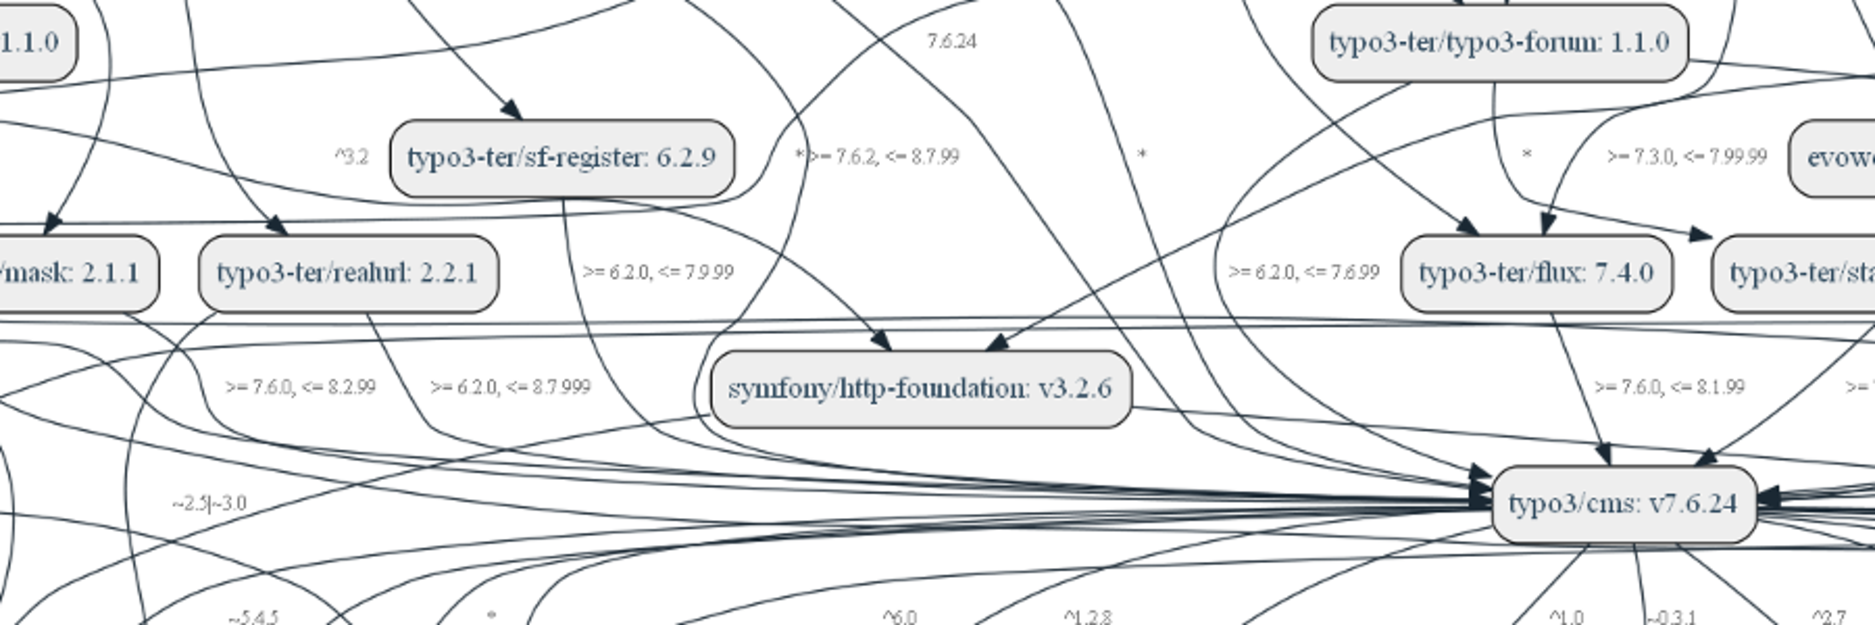
\includegraphics[
    width=\textwidth,
    height=\textheight,
    keepaspectratio
  ]{resources/dependency-graph.pdf}
  \caption{Ausschnitt des Gerichteter Graph für Abhängigkeiten der Individualsoftware}
  \label{dependency-graph}
\end{figure}

In Abbildung~\ref{dependency-graph} wird ein Ausschnitt der Abhängigkeiten der Individualsoftware dargestellt. Die vollständige Abbildung wäre zu umfangreich, um sie sinnvoll darzustellen. Zur Erstellung des Graphen wurde eine PHP-Bibliothek \glqq clue/graph-composer\grqq{} verwendet.

Die Betrachtung des vollständigen Graphen für beide Projekte, lässt Ähnlichkeiten erkennen. Auffällig bei beiden Projekten sind zentrale Knoten, also Abhängigkeiten die von vielen anderen Abhängigkeiten genutzt werden oder diese nutzen. Des weiteren könnten Gruppen von Abhängigkeiten ausgemacht werden. Solche Gruppen können ein eigenes, größtenteils abgrenzbares Abhängigkeitsnetz spannen. Damit dies möglich ist, müssten die Abhängigkeiten entsprechend gewichtet angeordnet sein. Im Falle des Graph-Composer-Werkzeuges erscheint dies nur mangelhaft zu gelingen. 

Abschließend sind in der Individualsoftware noch eine Reihe an unerwarteten Blattknoten erkennbar. Diese deuten auf schlecht gepflegte Abhängigkeiten hin. Unzureichende gepflegte Abhängigkeiten entstehen in der Regel, wenn die betroffenen Module nur im Gesamtkontext geprüft werden. Dadurch sind für diese Module implizite Abhängigkeiten verfügbar, die sonst nicht nicht bereitgestellt werden könnten.

\paragraph{Kreisdiagramm}

\begin{figure}[htbp]
  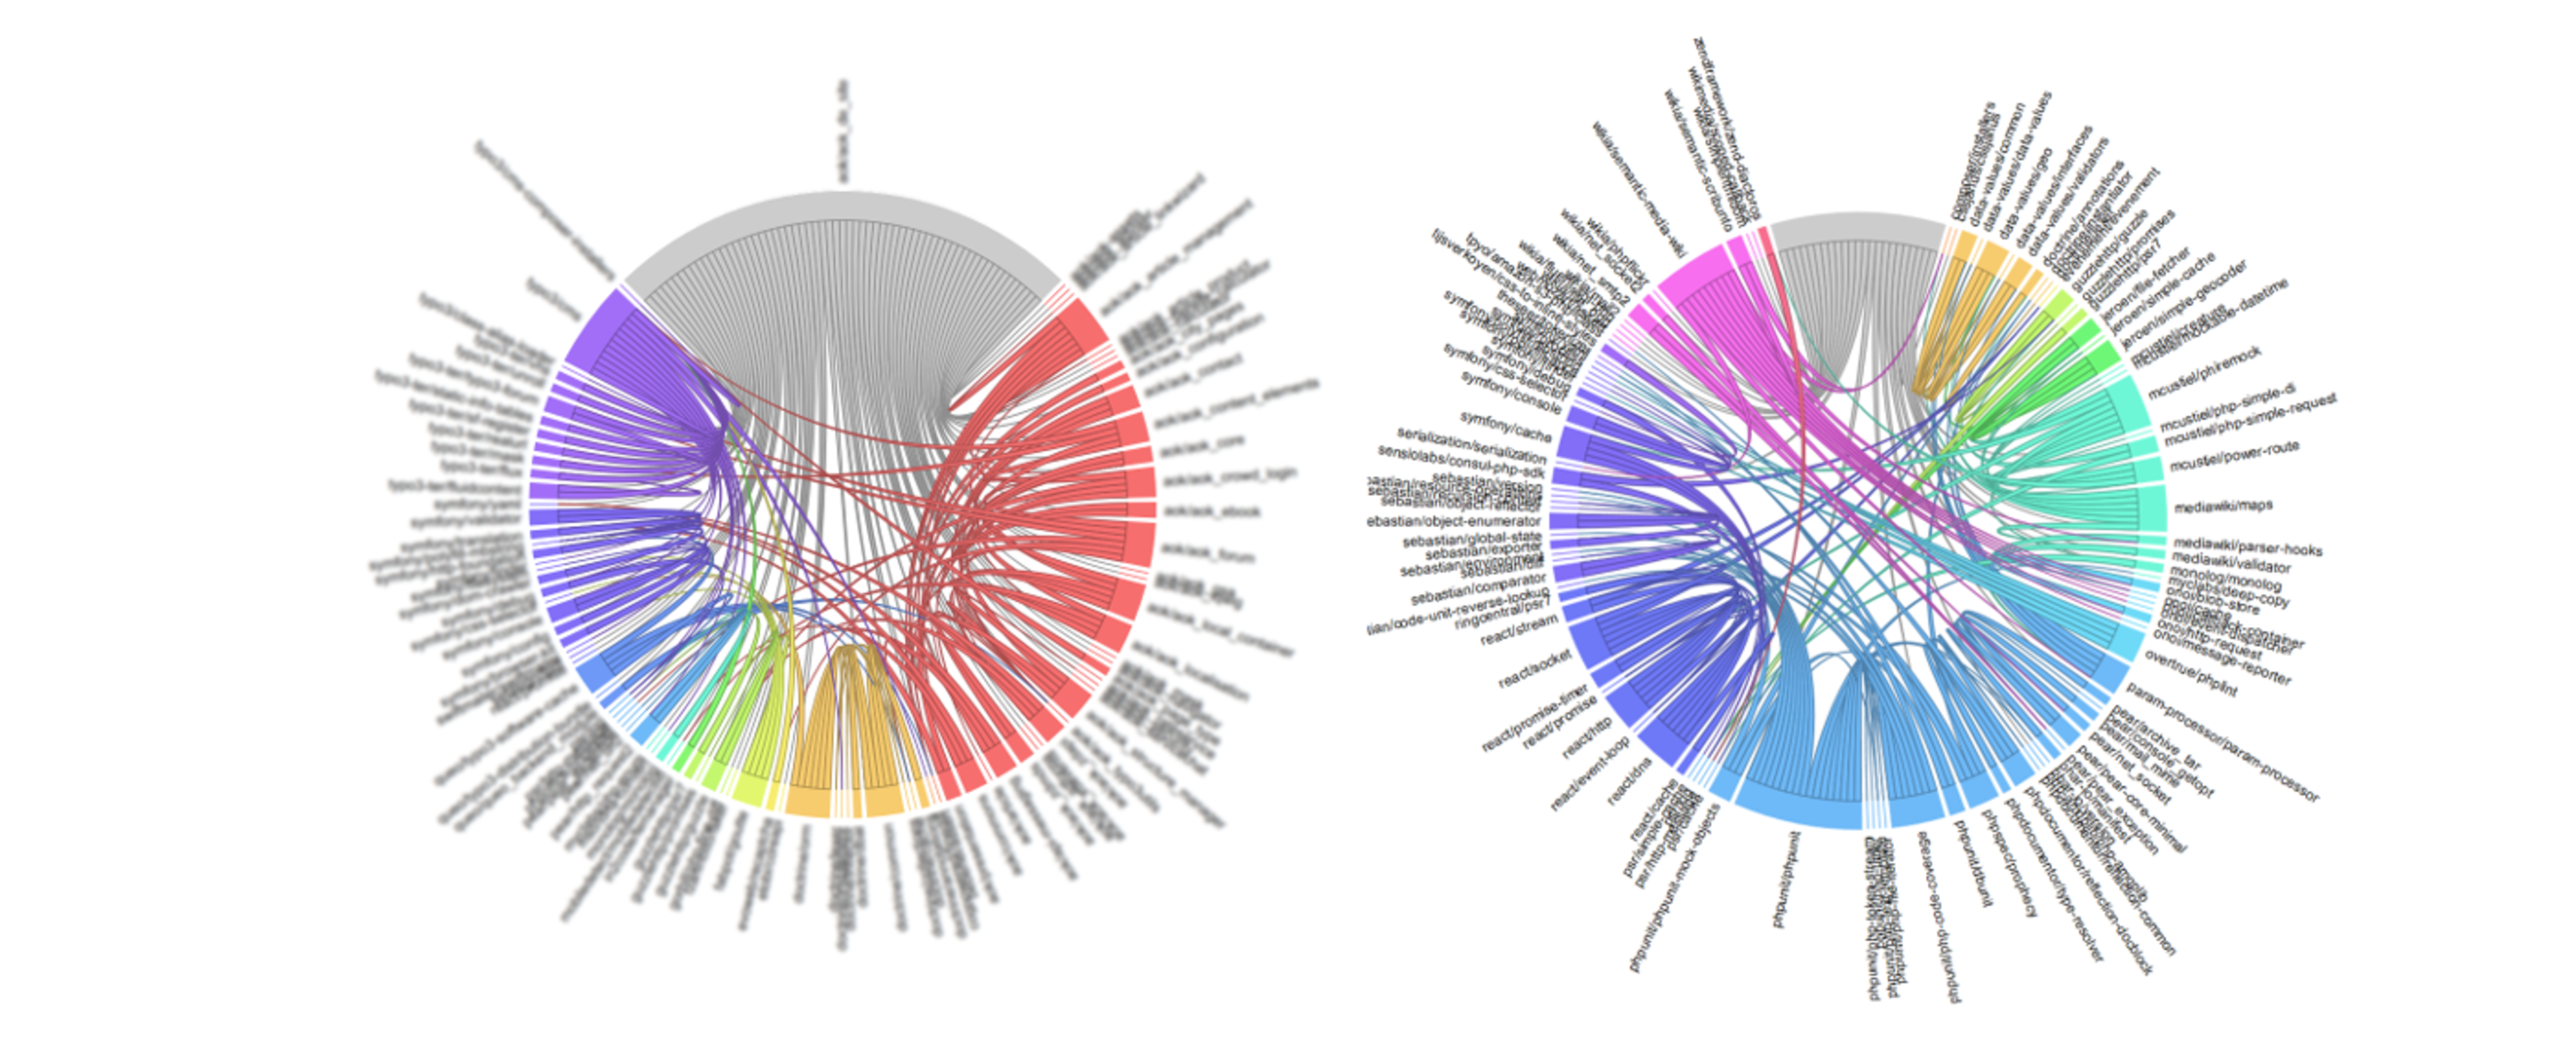
\includegraphics[
    width=\textwidth,
    height=\textheight,
    keepaspectratio
  ]{resources/circle-plot-dependencies.pdf}
  \caption{Kreisdiagramme für Abhängigkeiten}
  \label{dependency-circle-plot}
\end{figure}

In Abbildung~\ref{dependency-circle-plot} werden zwei Kreisdiagramme verwendet um die Abhängigkeitszu\hyp{} und abflüsse zu verdeutlichen. Das linke Diagramm stellt die Abhängigkeiten der Individualsoftware dar. Das rechte Diagramm visualisiert die Abhängigkeiten von Wikia. Die Wahl des Kreisdiagramms ergibt sich durch seine Eignung gruppierte Ab- und Zuströme zu visualisieren\footcite{visualizing-graph-data}. 

Als Basis für die beiden Diagramme wurden die im Versionsverwaltungssystem gesichert Dateien der Packetverwaltung verwendet. Das beschreibende Format ist eine DSL von Composer\footcite{composer-json} und wird primär für PHP-Projekte verwendet. Die Ansicht wurde mit Hilfe eines JavaScript-Werkzeuges \glqq Dependency Wheel\grqq{}\footcite{composer-dependency-wheel} erstellt.

Die grauen Abhängigkeitsteile stellen direkte Abhängigkeiten des Projektes dar, während die farbigen Stränge die Verbindungen der Abhängigkeiten visualisieren.

In der Darstellung der Individualsoftware, sind die roten Stränge interne Abhängigkeiten. Für Wikia sind Abhängigkeiten der eigenen Entwicklung Lila.

Beide Diagramme vermitteln einen guten Eindruck zur Fülle der Abhängigkeiten und eine Überblick darüber, wie viele Fremdabhängigkeiten im Projekt verwendet werden. Darüber hinaus sind allerdings nur schwer Informationen aus den sichtbaren Daten zu gewinnen. Zentrale Abhängigkeiten und Knoten lassen sich kaum ausmachen.

\subsection{Übersichten für Software-Metriken}

Metriken liefern diskrete Werte. Diese eigenen sich besonders für die maschinelle und automatisierte Verarbeitung. Sollen Entwickler anhand von Werten aus Metriken Entscheidungen treffen, stoßen diese schnell an kapazitive Grenzen. Visuelle Aufbereitungen dieser Werte helfen bei der Einordnung der Zahlen. Vergleiche zwischen Kenngrößen, Trends über Zeiträume und Gruppen von Werten lassen sich besser erfassen. Übersichtliche und gut aufbereitete Darstellungen helfen bei der Priorisierung und Bewertungen verschiedene Konstellationen. Abstrakte Sachverhalten wie Komplexität und Wartbarkeit können so erfasst werden.

\begin{figure}[htbp]
  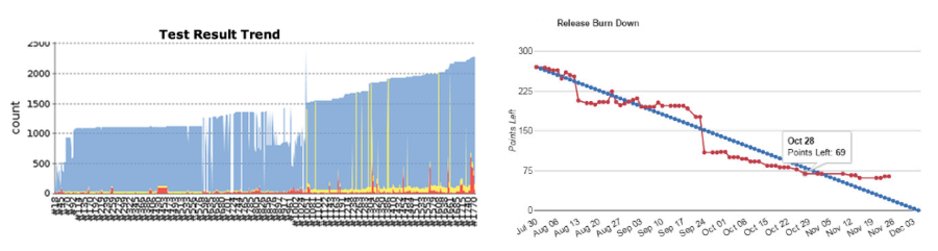
\includegraphics[width=\textwidth, height=\textheight, keepaspectratio]
    {resources/line-chart.pdf}
  \caption{Liniendiagramme für Testfälle(links) und verbleibende Aufwände(rechts)}
  \label{line-chart}
\end{figure}
\paragraph{Liniendiagramme} eignen sich besonders, um Trends und zeitliche Verläufe darzustellen. Zentrale und wichtige Größen, wie Testabdeckung, Komplexität, Kopplungsgrad können dadurch zeitlich betrachtet werden. Für bessere Sichtbarkeit können die Bereiche unter den Linien ausgefüllt sein.

Liniendiagramme eignen sich daher eher für langfristige Betrachtungen. Risikoabschätzung, Qualitätsentwicklung und Planung von Refactoring sind denkbare Einsatzgebiete.

\begin{figure}[htbp]
  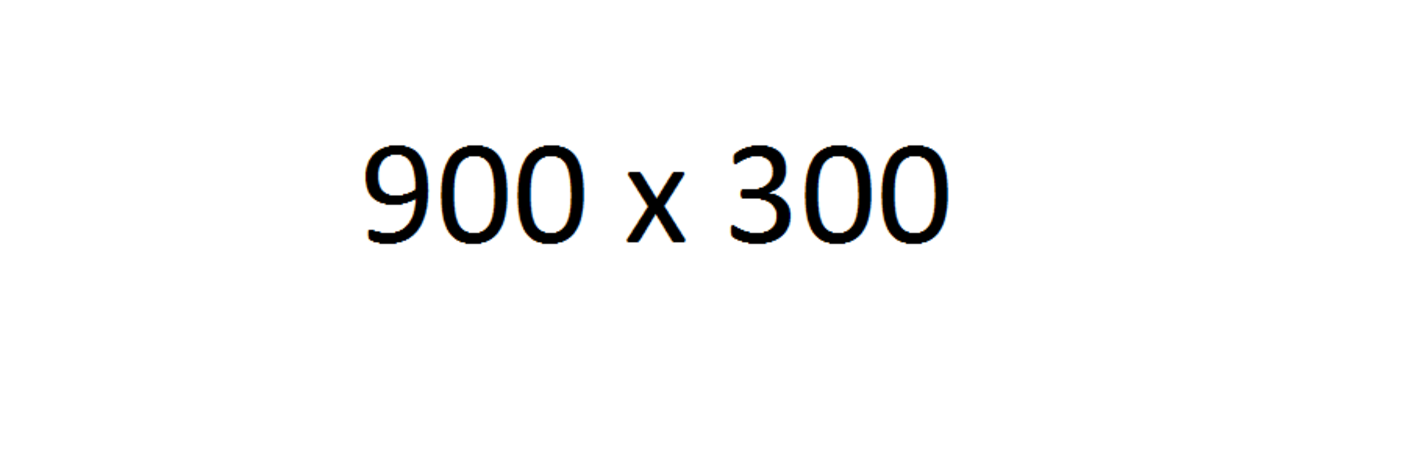
\includegraphics[width=\textwidth, height=\textheight, keepaspectratio]
    {resources/900x300.pdf}
  \caption{TODO Graphik zu Balkendiagrammen, horizontal, vertikal}
  \label{bar-chart}
\end{figure}
\paragraph{Balkendiagramme} eignen sich für vergleichende Ansichten. Kenngrößen können so in Kontext gesetzt werden. Die Vergleichsmöglichkeit erleichtert die Bewertung. Werden die Balken sortiert, können zudem Wertgruppen eingeteilt werden. Durch die Drehung des Balkendiagramms um 90 Grad, wird zudem der Fokus stärker auf die Sortierung gelenkt.

Balkendiagramme bilden Werte in einer gut vergleichbaren Form an. Dadurch eignen sie sich besonders für die Priorisierung und Gruppierung von Merkmalen.
Die Identifizierung der Gruppe der komplexesten Klassen oder die Gruppe der Klassen mit den meisten Abhängigkeiten können so schnell festgestellt werden. Mit Hilfslinien, parallel zu den Achsen, lassen sich gut Grenz- und Schwellwerte darstellen.

\begin{figure}[htbp]
  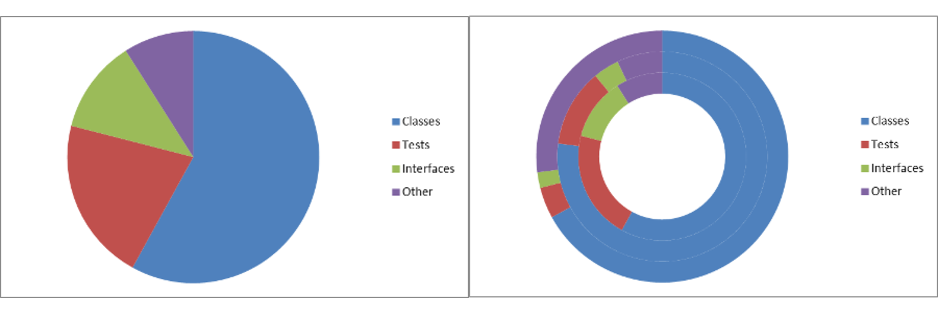
\includegraphics[width=\textwidth, height=\textheight, keepaspectratio]
    {resources/circle-graph.pdf}
  \caption{Bestandteile einer Abhängigkeit als Kreisdiagramm, Vergleich als Ringdiagramm}
  \label{circle-chart}
\end{figure}
\paragraph{Kreis- und Ringdiagramme} eignen sich gut um Zusammensetzungen darzustellen. Werden mehrere Zusammensetzungen als Ringdiagramme verschachtelt, lassen diese sich in Grenzen auch vergleichen. Kreisdiagrammen können verhältnismäßig schlecht kleinere Anteile darstellen. Unter anderem Beschriftungen können bei kleinen Teilen nur schwer dargestellt werden.

Besonders Verhältnisse zwischen Größen können mit Kreisdiagrammen gut dargestellt werden. Ähnlich zum Balkendiagramm, können sie sortiert und gruppiert Mehrheitsverhältnisse darstellen. Insbesondere Verhältnisse, die die Vertikale oder Horizontale Linie überschreiten, können gut argumentiert werden. So ist zum Beispiel die 50\% Marke in einem Kreisdiagramm eine gute Orientierungshilfe. Im Vergleich zum Balkendiagramm lassen sich diskrete Werte schwerer visualisieren.

\begin{figure}[htbp]
  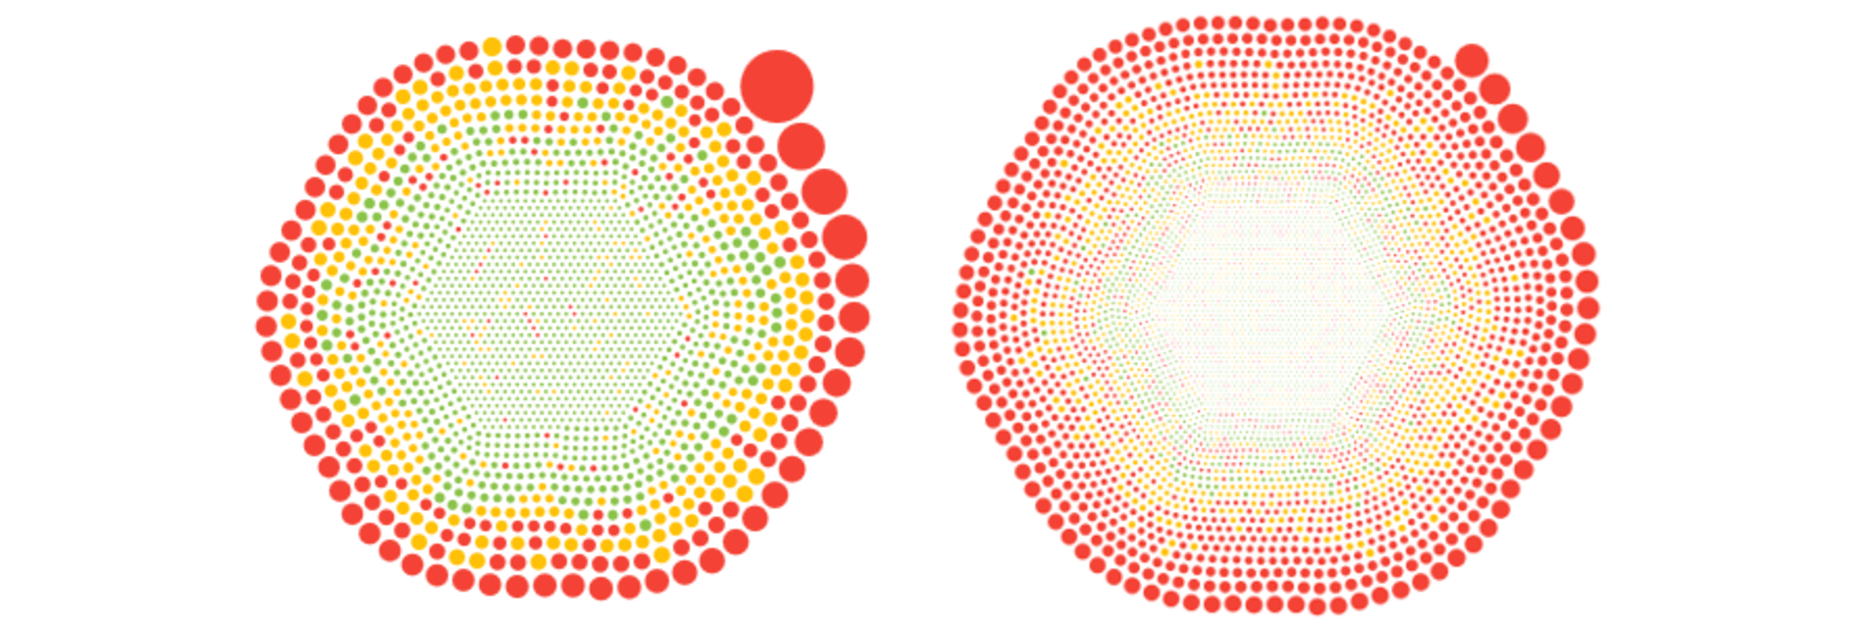
\includegraphics[width=\textwidth, height=\textheight, keepaspectratio]
    {resources/bubble-complexity-chart.pdf}
  \caption{Blasendiagramm für Zyklomatische Komplexität}
  \label{bubble-complexity}
\end{figure}
\paragraph{Blasendiagramme} eigenen sich besonders für die relative Darstellung von Werten. Oftmals werden die Blasen zusätzlich an den Achsen eines Graphen dargestellt. Im dargestellten Beispiel wurden die Blasen sortiert aufgereiht. Jede Blase steht im Beispiel für eine Klasse und die Größe der Blase für den Wert ihrer Zyklomatische Komplexität. Die Farbe der Klasse stellt einen Index für ihre Wartbarkeit zusammen. Die Darstellung ist eine Zusammenfassung der PHPMetrics\hyp{}Bibliothek. 
Die Darstellung vermittelt relativ einfach die Menge und Stärke von Komplexität und potentiellen Wartungsschwierigkeiten.


\section{Automatisierte Systembereitstellung}

Um Feature-Branches technisch zu unterstützen, müssen Tests und Metriken für jeden Feature-Branch ausgeführt werden. Damit dies automatisiert möglich ist, müssen die zugehörigen Testsysteme automatisch bereit stehen. Somit ist eine automatisierte Systembereitstellung notwendig.

Die automatische Bereitstellung ist prinzipiell, sowohl mit Virtualisierung, als auch mit einem Containersystem möglich. Auch eine halbautomatisch administrierte Gruppe an Hardwaresystemen ist möglich, sollte allerdings in den meisten Situation deutlich unwirtschaftlicher sein als die virtuellen Lösungen.

Die Entscheidung für eine Virtualisierungs- oder Containerlösung sollte von Fall zu Fall getroffen werden. Die schlankere und damit Resourcen schonendere Lösung, ist die Verwendung von Containern. Mit ihnen können problemlos einzelne Testsysteme oder komplexere Service und Systemverbände erstellt und verwaltet werden. Die Verwendung eines einzelnen Container-Systems ist nicht mehr möglich, wenn unterschiedliche Betriebs- oder Hardwaresysteme benötigt werden. In diesem Fall müssen mehrere Container-Systeme konfiguriert werden.

Unabhängig von der verwendeten Lösung, müssen die Systeme in einen definierten Zustand geführt werden. Dieser Vorgang kann einen größeren Zeitraum in Anspruch nehmen und benötigt entsprechende manuelle Resourcen. Um diesen Zeitraum zu verringern, sollten anhand des Konfigurationsmanagements exemplarische Systeme vorbereitet und in gepackter Form abgelegt werden. Bei den meisten Lösungen wird diese Form \glqq Image\grqq{} genannt. Wie bereits bei \glqq Artefakt-Repositories\grqq{} angesprochen, sollten diese Images nachvollziehbar benannt und abgelegt werden. Es sollte möglich sein eine Verbindung zur jeweiligen System-Konfiguration herzustellen. Bestenfalls ist die System-Konfiguration in einer Versionsverwaltung abgelegt und die entsprechende Version kann ebenfalls zur Referenzierung des System-Images verwendet werden. Um die Übereinstimmung mit den verknüpften Übersichten zu gewährleisten, ist es sinnvoll diese im Rahmen der automatischen Systembereitstellung zu aktualisieren. Übersichten wie die Konfigurations\hyp{} und Systemübersicht aus Kapitel~\ref{subsubsec:configuration-system-overview} sollten stets aktuell sein.

\section{Best Practices in der Softwareentwicklung}

Feature-Branches verhindern keine Merge-Konflikte, die beim Zusammenführen von Änderungen auftreten. Sie helfen lediglich, das Auftreten der Konflikte, zu einem gewählten Zeitpunkt zu verschieben. Daher sind Entwickler, auch mit Features-Branches, darauf angewiesen Entwicklungsmuster anzuwenden und sich mit der Softwarearchitektur der Softwareanwendung auseinanderzusetzen.

Zudem unterstützen die nachfolgenden Methodiken das Verfahren \glqq \nameref{temporary-releases}\grqq{} aus Kapitel~\ref{temporary-releases}. Das Verfahren ist abhängig von Code-Kopplung und profitiert von einer besseren Testqualität.

Viele dieser Entwicklungsmuster und -verfahren werden unter dem Begriff \glqq Best Practices\grqq{} geführt. Sie unterstützen Entwickler in Entwurfsentscheidungen und geben Rahmen für Standards in der Softwareentwicklung. Viele der Best-Practices zielen zudem auf Verbesserungen für Wartbarkeit, Robustheit und allgemeine geringere Umsetzungsaufwände.

\subsection{Modularisierung von Software}

Viele Probleme bei Continuous-Integration und Feature-Branches entstehen durch Merge-Konflikte. Diese Merge-Konflikte müssen in teilweise sehr komplizierten Merge-Verfahren aufgelöst werden. Merge-Konflikte treten auf, wenn Änderungen aus verschiedenen Commits die gleichen Dateien betreffen. Besonders bei Komponenten der Softwareanwendung, die stark gekoppelte Abhängigkeiten verwenden, treten Merge-Konflikte besonders häufig auf. Wird eine Software von Beginn an lose gekoppelt entwickelt, ergeben sich oft deutlich weniger Abhängigkeiten und komplizierte Merge-Schritte werden vermieden.

Die lose Kopplung einer Software kann, durch das Befolgen der Prinzipien zur Modularisierung\footcite{2012-barth-modularisation}, erreicht werden. 

\paragraph{Information Hiding} ist ein von Parnas\footcite{1972-parnas} geprägter Begriff. Als Basis für die Modularisierung und Dekomposition von Software wird drei Schritten gefolgt:
\begin{itemize}
\item Ermittle alle Entwurfsentscheidungen, welche sich potentiell ändern werden.
\item Erstelle pro Entwurfsentscheidung ein Modul, die Entwurfsentscheidung wird \glqq Geheimnis des Moduls\grqq{} genannt.
\item Die Schnittstelle zum Modul sollte robust genug sein, um bei einer Änderung des Geheimnisses nicht verändert zu werden.
\end{itemize}
Durch die Einhaltung der Prinzipien, werden mögliche Änderungen auf ein Modul beschränkt und damit die Auswirkungen begrenzt.
\paragraph{Separation of Concerns} ist ein Basisprinzip moderner Softwareentwicklung. Während Information-Hiding auf einer niedrigen Modulebene ansetzt, versucht die \glqq Aufteilung nach Anliegen\grqq{} höher anzusetzen. Die Teile eines Moduls sollen nach möglich Anliegen  mit möglich wenig Überlappungen eingeteilt werden.
\paragraph{Low Coupling Cohesion} beschreibt das Verbindungs- und Kommunikationsverhalten der Module. Es wird eine hohe Kohäsion innerhalb eines Moduls angestrebt und eine geringe zu anderen Modulen.

Werden die Prinzipien befolgt, ergeben sich Vorteile für die Wartbarkeit, Wiederverwendbarkeit und Robustheit der Softwareanwendung. 

Eine modernere Form der Modularisierung sind die \glqq serviceorientierten Architekturen\grqq{}. Diese beschreiben Anwendungsszenarien in verschiedenen Granularität. Die Kapselung in Services ermöglichen die Komposition und Orchestrierung von komplexen Vorgängen. Der serviceorientierte Ansatz nutzt die Prinzipien der Modularisierung und bietet die Vorteile unter neuem Namen an.

\subsection{Testgetriebene Entwicklung}
\label{test-driven-development}

Testgetriebene Entwicklung, oder auch Test-Driven-Development(TDD) wurde bereits von Kent Beck 1999 als \glqq test-first\grqq{}-Ansatz propagiert. Seitdem hat dieses Vorgehen viele Anhänger gewonnen. Es fordert ein Umdenken beim Entwickler. Zuerst muss das Ergebnis einer Änderung oder einer Neuerung bekannt sein und erst danach kann der umsetzende Code entwickelt werden\footcite[vgl.][Kap. Understanding TDD]{tdd-java}. Die Umkehrung des Zeitpunktes, wann die Tests verfasst werden, fördert die Qualität der Entwicklung. Es werden die Anzahl der auftretenden Fehler reduziert, entkoppelte Strukturen gefördert und die Anzahl der nachträglich auftretenden Fehler deutlich gemindert\footcite[vgl.][]{tdd-ci-effectivness}.
Insbesondere im Continuous-Integration-Bereich ist TDD als Continuous-Testing sinnvoll, da nur kontinuierlich getesteter Code auch kontinuierlich zuverlässig integriert werden kann.

Die Art und Weise der Anwendung von TDD kann stark variieren. Daher wird eine stark iterative Variante des Schreibens von Tests angestrebt. Das \glqq Red Green Refactoring\grqq{}\footcite[vgl.][Kap. Red-Green-Refactor]{tdd-java} fordert immer nur minimale Anpassungen vorzunehmen, bis der Test vollständig ist. Nach jeder Anpassung, die den Test fehlschlagen lässt, muss die getestete Implementierung so angepasst werden, dass der Test erfolgreich verläuft. Ist der Test vollständig, sollte abschließend die Implementierung einem Refactoring unterzogen werden. Basierend auf der begrenzten gedanklichen Kapazität eines Entwicklers, soll immer nur ein Gesichtspunkt der Entwicklung betrachtet werden. Zuerst soll das korrekte Verhalten der Software sichergestellt werden. Danach ist die korrekte Struktur der Software herzustellen. Die Dualität der Betrachtung und der minimal inkrementelle Ansatz sollen ein hoch qualitatives Resultat ergeben.

Über die Lehrmethoden von TDD sind bekannte Verbindungen von Anforderungsmanagement und Testfallerstellung, wieder in den Fokus gerückt. Unter der Bezeichnung \glqq Behaviour-Driven-Development\grqq{}\footcite{bdd-north} entstand ein Verfahren zur Verbindung beider Bereiche. Mittels einer der Umgangssprache nahen DSL wird versucht eine leserliche Dokumentation zu erstellen. Nutzerszenarien werden in einer Gegeben-Wenn-Dann-Notation\footcite{fowler-gwt} verfasst und können durch die strukturierte Notation direkt mit Test-Code verknüpft werden. Damit wird angestrebt die Barrieren zwischen Projektteilnehmern ohne Programmierkenntnissen, Testern und Entwicklern zu verringern.

Neben dem Erfolg von TDD wurde auch Kritik geäußert. Unter anderem wurde der starke Fokus auf Unit-Tests kritisiert. Dieser soll in der Historie von TDD begründet sein\footcite[vgl.][]{conciso-tdd-critique}. Der Fokus auf Unit-Tests wird kritisiert, da der Fokus auf die Integration von Komponenten verloren geht und die Funktionalität des Systems nicht überprüft wird. Weiter wird kritisiert, dass TDD schlechtes Design fördert\footcite[vgl.][]{hansson-tdd-is-dead}. Das Prinzip die Softwareanwendung leicht zugänglich für Tests zu gestalten, soll die Architektur nachhaltig schädigen.

Die Kritik weist Schwächen auf. TDD fordert die Erstellung von Tests. Die Begrenzung der Tests auf Unit-Tests wird allerdings an keiner Stelle gefordert. Der ursprüngliche Test-Frist Ansatz von Kent Beck ist besonders Intuitiv, wenn er für Unit-Tests verwendet wird. Die Annahme, dass er auf Unit-Tests beschränkt wird, würde TDD allerdings nicht gerecht. 

Weiter ist eine sehr subjektive Einschätzung, dass TDD die Softwarearchitektur schwächt. Eine zu strikte Befolgung aller Prinzipien von TDD oder Modularisierung kann zu ungünstigen Entscheidungen im Software-Design führen. Die Korrekte Anwendung der Prinzipen liegt daher in der Hand des Entwicklers. In einer kritischen Auseinandersetzung von Kent Beck, Martin Fowler und David Heinemeier Hansson zum Thema TDD, formuliert Kent Beck die folgende Aussage:

\blockquote {Design(and TDD) is a question of trade–offs. They should never be ignored. You should always be aware of the trade–offs you make. You have to be a good designer to make the right ones.}\footcite[vgl.][S. 36]{aalborg-tdd-15-years}

Test-Driven-Development ist sinnvoller Ansatz um nachhaltig hochqualitativen Software-Code zu verfassen. TDD fördert durch den Fokus auf gut zu testenden Software-Code lose gekoppelte Software-Komponenten. Allerdings entbindet das TDD-Vorgehen den Softwareentwickler nicht von den zu treffenden Softwarearchitekturentscheidungen.

\subsection{Fortgeschrittene Nutzung von Versionsverwaltung}

Die Versionsverwaltung ist nicht nur eine Ablage für Quellcode, sondern auch Teil der Dokumentation eines Projektes. Daher ist es wichtig die veröffentlichten und geteilten Änderungen zu strukturieren. In einem ideal Szenario besteht jeder Commit nur aus einer sehr kleinen, nur eine Datei betreffenden Änderung, die durch eine Aussagekräftige Commit-Message in Kontext gesetzt wird\footcite[vgl.][Kap. Making only one change per commit]{git-essentials-2017}. Eine Folge von zusammenhängenden Änderungen sollte zudem ein gemeinsames Label teilen. Dieses kann später für Filterungen verwendet werden. Dadurch ist es auch lange Zeit später möglich zusammenhängende Commits zu finden.

Wird ein zentrales Versionsverwaltungssystem zusammen mit Continuous-Integration verwendet, ist außerdem die Build-Integrität sicherzustellen. Keiner der Commits sollte den Build fehlschlagen lassen. 

Die Verwendung einer dezentralen Versionsverwaltung und Feature-Branches erleichtert das Erstellen von Commits. Zum eine ist die Build-Integrität abgeschwächt. Dies ermöglicht es, zugunsten eines einfache Commits, die Build-Integrität erst mit den nachfolgenden Commits herzustellen. Zum anderen lassen sich in einer dezentralen Versionsverwaltung die Commits nachträglich verändern. Dies ermöglicht die Commits unter Umständen verständlicher zu strukturieren.

Eine Variante verständliche und gut strukturierte Commit-Nachrichten zu verfassen, ist es die Commit-Nachrichten vor der Implementierung der Änderung zu verfassen\footcite[Writing commit messages before starting to code][]{git-essentials-2017}. Ähnlich wie in Kapitel~\ref{test-driven-development}~\nameref{test-driven-development}, wird der Fokus auf das Ergebnis, nicht die Implementierung gelenkt. Es wird somit beschrieben, welches Ziel der Commit verfolgt, nicht welche Änderungen durchgeführt wurden. Die dokumentierenden Qualitäten der Versionhistorie werden dadurch deutlich verbessert.

\subsection{Verwendung von Monorepo-Repositories}

Im Abschnitt~\ref{subsubsec:illustrate-dependencies}~\glqq \nameref{subsubsec:illustrate-dependencies}\grqq{}, konnten gut Abhängigkeitsgruppierungen erkannt werden. Gerade bei Abhängigkeitskonstrukten innerhalb einer Organisation, werden häufig Änderungen parallel in mehreren Abhängigkeiten vorgenommen. Gerade wenn sich diese Abhängigkeiten gegenseitig bedingen, kann es zu einem erhöhten Aufwand kommen. Damit ein gemeinsamer Stand erreicht wird, müssen häufig mehrere Teile des Projektes aktualisiert werden. Gerade wenn ein experimentelles Feature auf mehreren zusammenhängenden Feature-Branches getestet werden muss, entsteht ein deutlich erhöhter Aufwand.

Eine Variante diese Aufwände zu reduzieren und Tests, sowie Auslieferung von Software für ein Paket von Abhängigkeiten zu optimieren, sind Monorepos. Monorepos verwenden, im Kontrast zu regulären Praktiken, ein Repository für mehrere Abhängigkeiten\footcite{trunkbaseddevelopment-monorepo}. Dieses Vorgehen hat den direkten Vorteil, dass Abhängigkeiten nicht miteinander verlinkt werden müssen. Abhängigkeiten sind durch das gemeinsam geteilte Repository automatisch verbunden. Zudem können gemeinsam verwendete Werkzeug einfach gleichgeschaltet und die gemeinsame Verwendung begünstigt werden.

Die Verwendung eines Monorepos vereinfacht zwar die Abhängigkeitsverwaltung, birgt allerdings Schwierigkeiten für größere Repositories. Während in Repositories getrennte Abhängigkeiten, auch die Commits logisch und physisch getrennt sind, fällt diese Barriere in Monorepos. Es müssen daher zusätzliche Mechanismen für die Übersicht geschaffen werden.

Ein weiterer Punkt ist die Performance. Abhängig vom gewählten Versionsverwaltungssystem, können gerade durch die Verwendung von Git Probleme auftreten. Da Git immer die vollständige Historie bereit hält, sind Performance-Probleme nachweisbar\footcite{atlassian-monorepo-git}. In zentralen Systemen wie SVN können für Monorepos gezielte Teilebereiche des Repos verwendet werden. 
In jedem Versionsverwaltungssystem ist hingegen die erhöhte Commit-Frequenz spürbar. Merge-Commits treten deutlich häufiger auf, zusätzliche manuelle Eingriffe sind teilweise notwendig.

Trotz der Schwierigkeiten nutzen große Unternehmen wie Google, Facebook und Twitter sehr große Monorepos. Für alle drei Unternehmen ist die Verwendung von Monorepos allerdings mit großem Aufwand verbunden. Google entwickelte eine eigene Versionsverwaltung, Facebook investiert in Mercurial und Twitter verwendet eine speziell angepasste Git-Variante\footcite{monorepos-wild}.
Bei entsprechender Größe des Projektes, ist allerdings auch für kleinere Unternehmen die Verwendung von Monorepos nützlich\footcite{hackernoon-positive-monorepo}.

\section{Umfrage zum Nutzungsverhalten von Versionsverwaltungssystemen und Tests}
\label{survey-vcs-test}

Um die Verwendung von Versionsverwaltung und die Anwendung von Tests in Kontext setzen zu können, wurde ein Umfrage durchgeführt.
Ziel der Umfrage ist es mögliche Schwächen und Mängel im Umgang mit Versionsverwaltung und Tests aufzudecken. Weiter wird versucht mögliche Korrelationen zwischen spezifischen Versionsverwaltungssystemen und spezifischen Tests zu erkennen.

Die Umfrage wurde ausschließlich als Online-Umfrage durchgeführt. Als Umfrage Werkzeug wurde die selbst gehostete Open-Source-Anwendung \glqq LimeSurvey\grqq{}\footcite[][]{limesurvey} verwendet. Über einen Zeitraum von einem Monat konnten Teilnehmer den Fragebogen ausfüllen. Die Umfrage wurde über soziale Medien verteilt und einem Verteiler innerhalb einer Firma.

Die Umfrage enthielt 33 Fragen in 3 Fragegruppen. Der erste Teil erhob Daten zur Einordnung des Teilnehmers. Der zweite Teile beschäftigte sich mit der Nutzung von Versionsverwaltung und der abschließende dritte Teil mit der Verwendung von Tests.

Über den Umfragezeitraum sind 185 Antworten angefangen worden. Davon enthielten 46 Antworten verwertbare Ergebnisse, aber nur 29 Antworten wurden vollständig abgeschlossen. Die weit auseinander gehenden Zahlen lassen auf mögliche technische Schwierigkeiten schließen.

Der Großteil der Fragen bedient sich einer fünf-geteilten Likert-Skala. Zudem ist möglich Antworten zu ignorieren, daher ist der Auswertung eine sechste spalte sichtbare. Das parametrische Verfahren  der Likert-Skala bietet deutliche Vorteile bezüglich der Zusammenfassung und Auswertung der Antworten. Die Likert-Skala setzt voraus, dass die Antwortmöglichkeiten einen gleichen Abstand zueinander aufweisen. Weiter wird eine Normalverteilung unter den Teilnehmern vorausgesetzt. 

Die Umfrage wurde in einer spezifischen Firma verbreitet und die Teilnehmerzahl ist deutlich unterhalb einer repräsentativen Menge geblieben. Beide Faktoren lassen die Vermutung zu, dass keine Normalverteilung unter den Teilnehmern gegeben sein wird. Die Ergebnisse sind daher nur sehr begrenzt anwendbar.

Auch der konstante Abstand der Antworten ist nicht sichergestellt. Die Abfolge der Antworten wird unter Umständen nicht von jedem Teilnehmer als gleichwertige Abstufung wahrgenommen.

\subsection{Teilnehmerzusammensetzung}

\begin{figure}[htbp]
  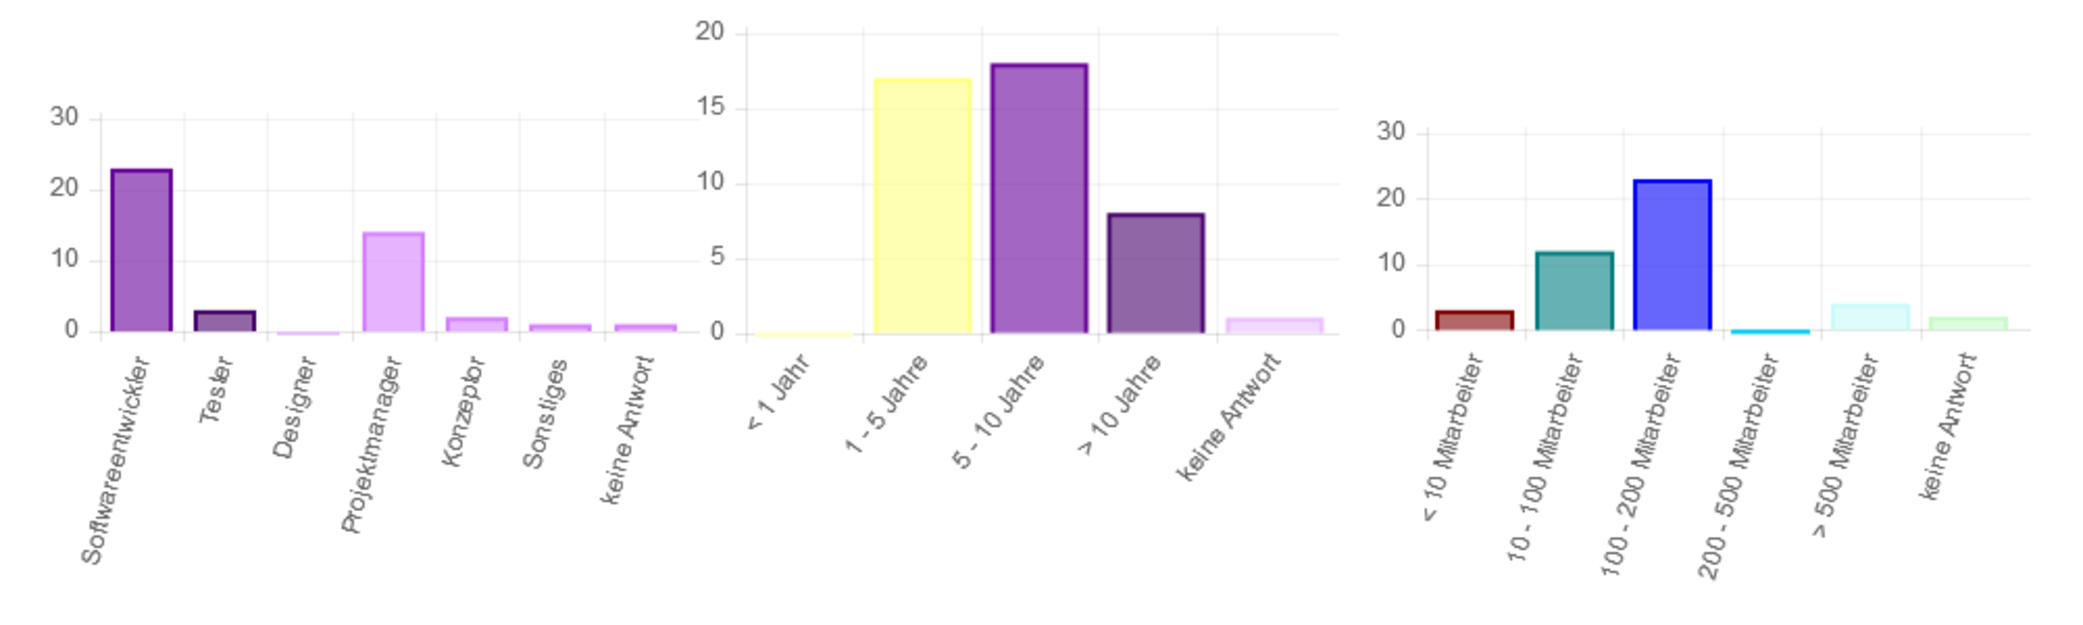
\includegraphics[width=\textwidth, height=\textheight, keepaspectratio]
    {resources/survey-participants.pdf}
  \caption{Auswertung zur Teilnehmerzusammensetzung (Tätigkeit, Erfahrung, Firmengröße}
\end{figure}
Die auswertbaren Umfrageteilnehmer gaben größtenteils an Softwareentwickler oder Projektmanager zu sein. Weiter sind die Gruppen mit 1-5 Jahren und 5-10 Jahren Berufserfahrung am stärksten vertreten. Abschließend ist noch die Zusammensetzung der Firmengrößen hervorzuheben. Der größte Teil der Teilnehmer gab an in kleinen und mittelständischen Unternehmen zu arbeiten.

Die Gruppe der Softwareentwickler wird teilweise explizit hervorgehoben, als besonders relevante Gruppierung für das Thema.

\subsection{Nutzung von Versionsverwaltung}

\begin{figure}[htbp]
  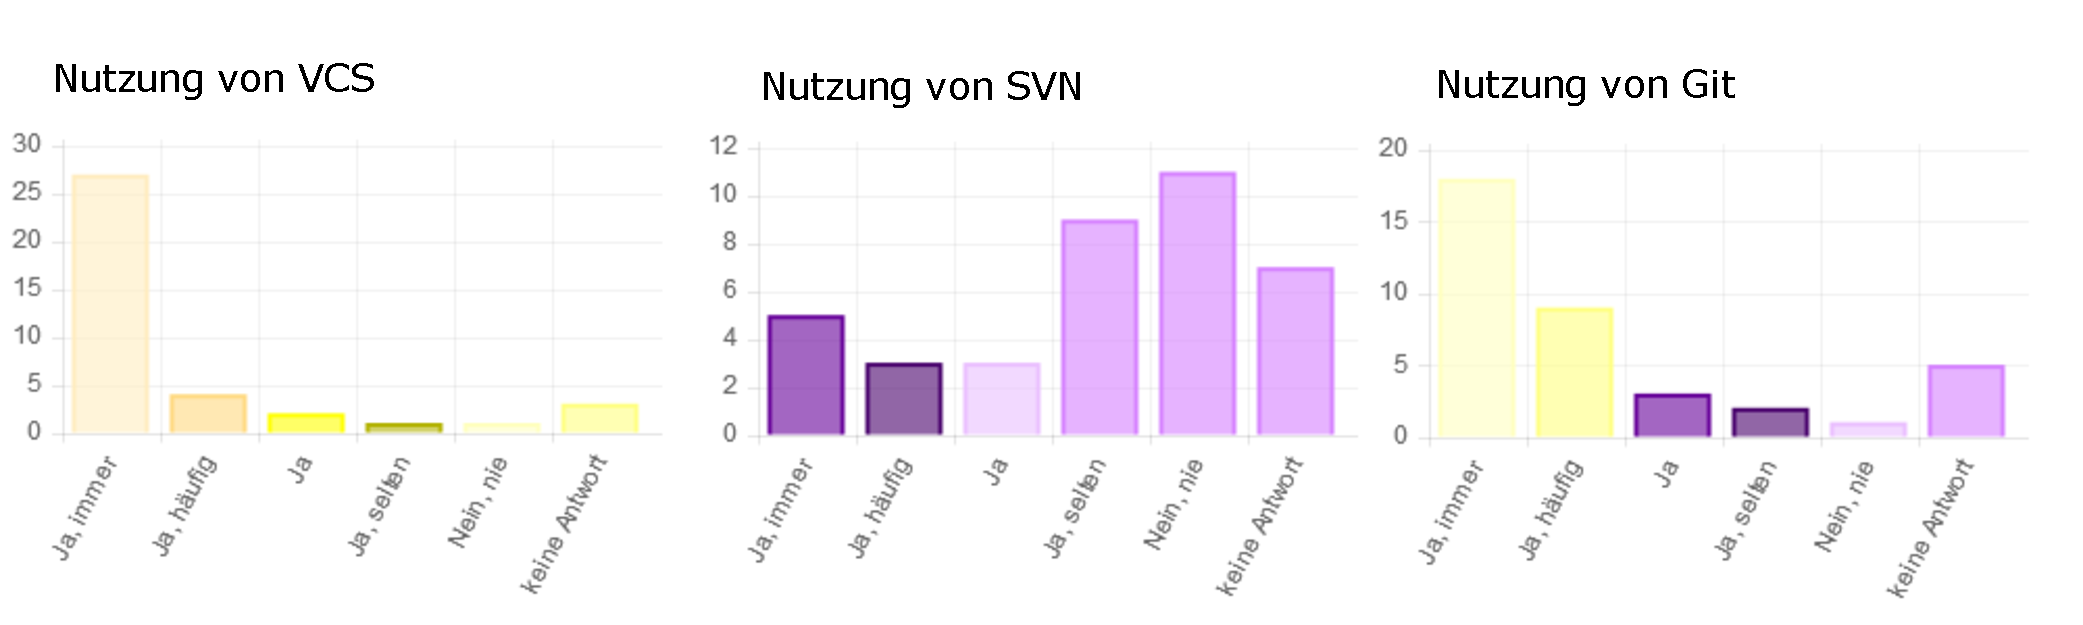
\includegraphics[width=\textwidth, height=\textheight, keepaspectratio]
    {resources/survey-vcs-usage.pdf}
  \caption{Auswertung der Versionsverwaltung (Gesamt, SVN, Git)}
\end{figure}

\paragraph{Generelle Verwendung}

Die Verwendung einer Versionsverwaltung wurde von 88\% angegeben. Im Gegensatz zu den in  Kap.~\ref{distributed-vcs-git} aufgeführten Statistik, wird hautsächlich Git verwendet. Bezogen auf die Umfrageteilnehmer, welche eine Versionsverwaltung nutzen, gaben 94\% der Umfrageteilnehmer an Git zu verwenden. 58\% Gaben an Subversion zu verwenden, allerdings selten (26\%). 

Bezogen auf die Gruppe der Softwareentwickler, wurde von jedem angegeben eine Versionsverwaltung zu nutzen, allerdings ignorierten fast 20\% die Frage. 91\% der Softwareentwickler gaben an Git zu verwenden. Weiter gaben 52\% der Softwareentwickler an Subversion zu verwenden.

\begin{figure}[htbp]
  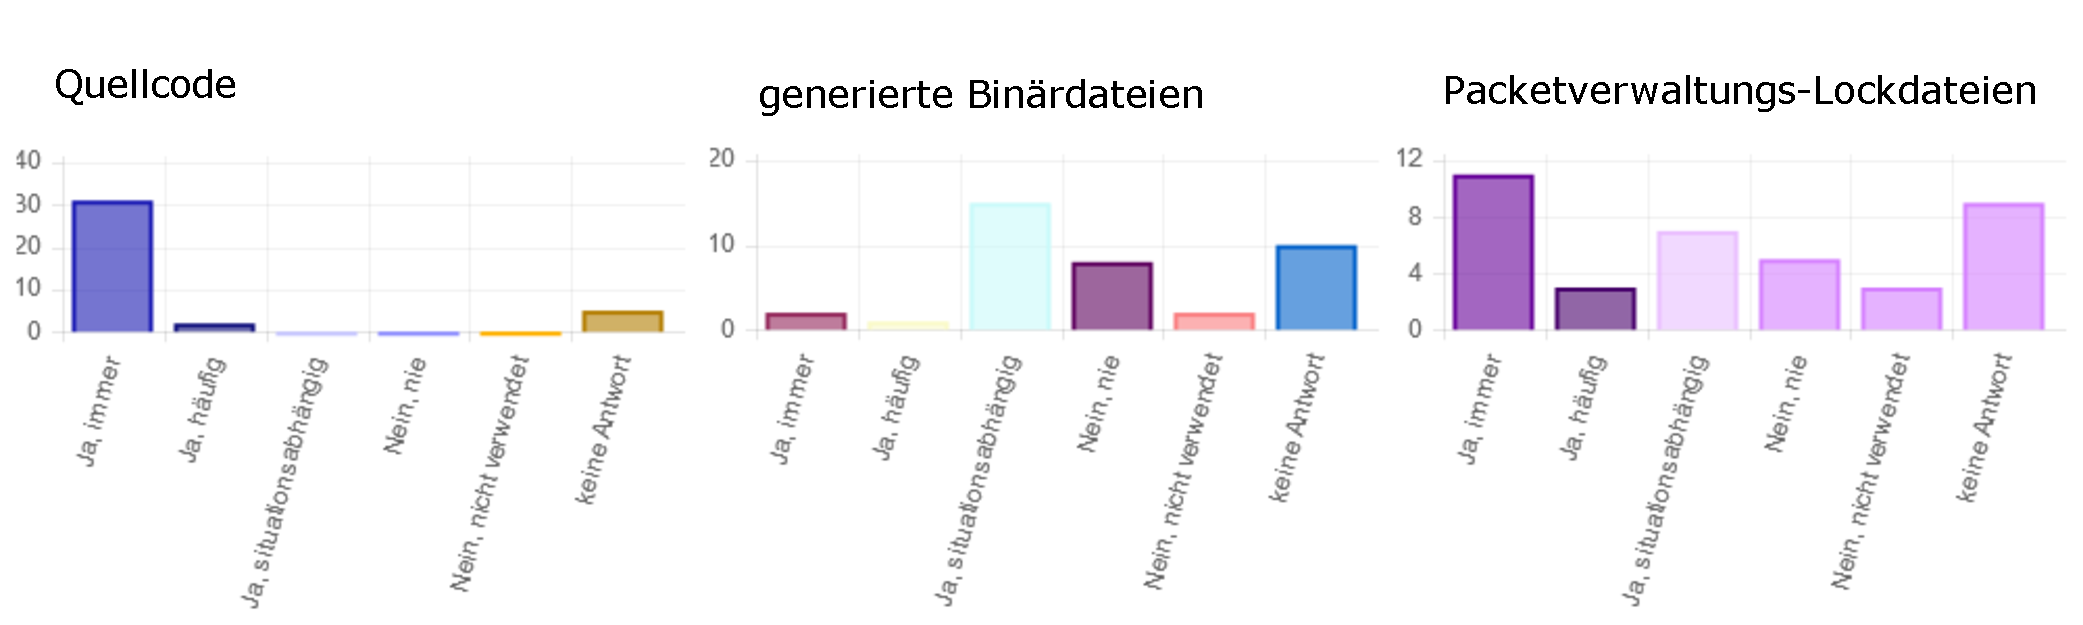
\includegraphics[width=\textwidth, height=\textheight, keepaspectratio]
    {resources/survey-vcs-content.pdf}
  \caption{Auswertung der Abgelegten Inhalte (Quellcode, Binärdateien, Packetverwaltungsdateien)}
\end{figure}

\paragraph{Inhalte unter Versionsverwaltung}

Dateien und Inhalte die in der Versionsverwaltung abgelegt werden, wurden von den Teilnehmern großteils als nicht-binär angegeben. Quelltexte werden von (97\%) der Teilnehmer abgelegt. Build-Skripte(85\%) und Migrations-Skripte(91\%) werden ebenfalls vom Großteil versioniert. Die Mehrheit der Teilnehmer verwendet die Versionsverwaltung nur für kleine Mediendateien (79\%) und kein größeren (62\%).

Während für die meisten Dateien und Inhalte sich deutliche Muster ergaben, war die Ablage von Packetverwaltungs-Lockfiles oder anderen Build-Identifikations-Dateien nicht eindeutig. Betrachtet auf die Menge der Entwickler, nutzen 22\% keine Versionsverwaltung für diesen Dateityp.

\paragraph{Verwendung von Branches und Tags}

\begin{figure}[htbp]
  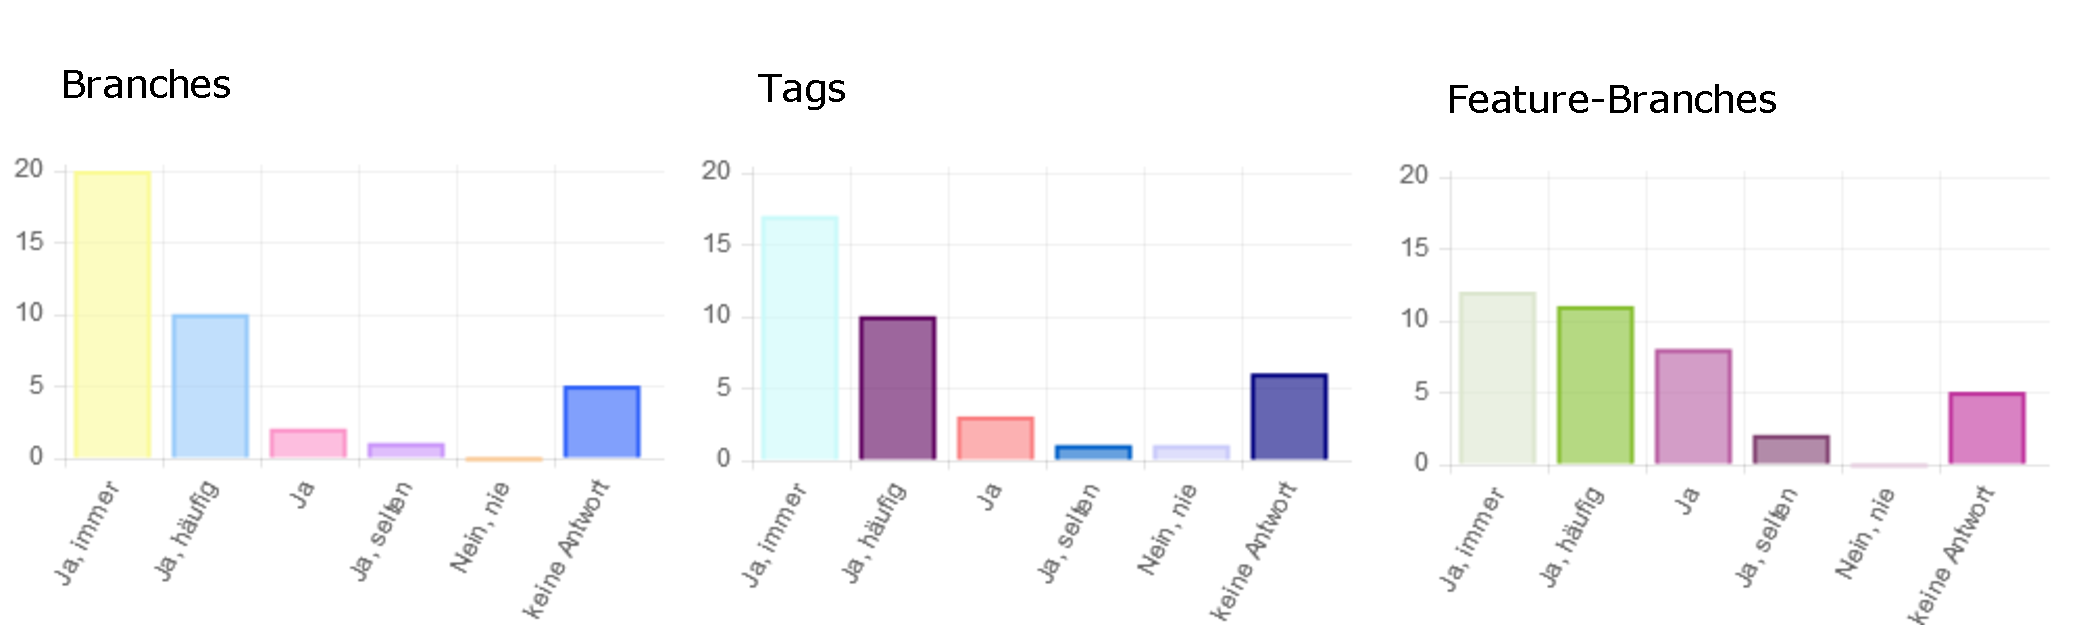
\includegraphics[width=\textwidth, height=\textheight, keepaspectratio]
    {resources/survey-vcs-branches.pdf}
  \caption{Auswertung der Verwendung von Branches, Tags und Feature-Branches}
\end{figure}

Branches(97\%) und Tags(91\%) werden grundsätzlich verwendet. Die Verwendung von Feature-Branches ist durchweg zu verzeichnen, aber korreliert weniger mit der grundsätzlichen Verwendung von Branches. Die hohe Nutzung von Branches korreliert mit der generellen Verwendung von Git.

\paragraph{Merge-Konflikte}

\begin{figure}[htbp]
  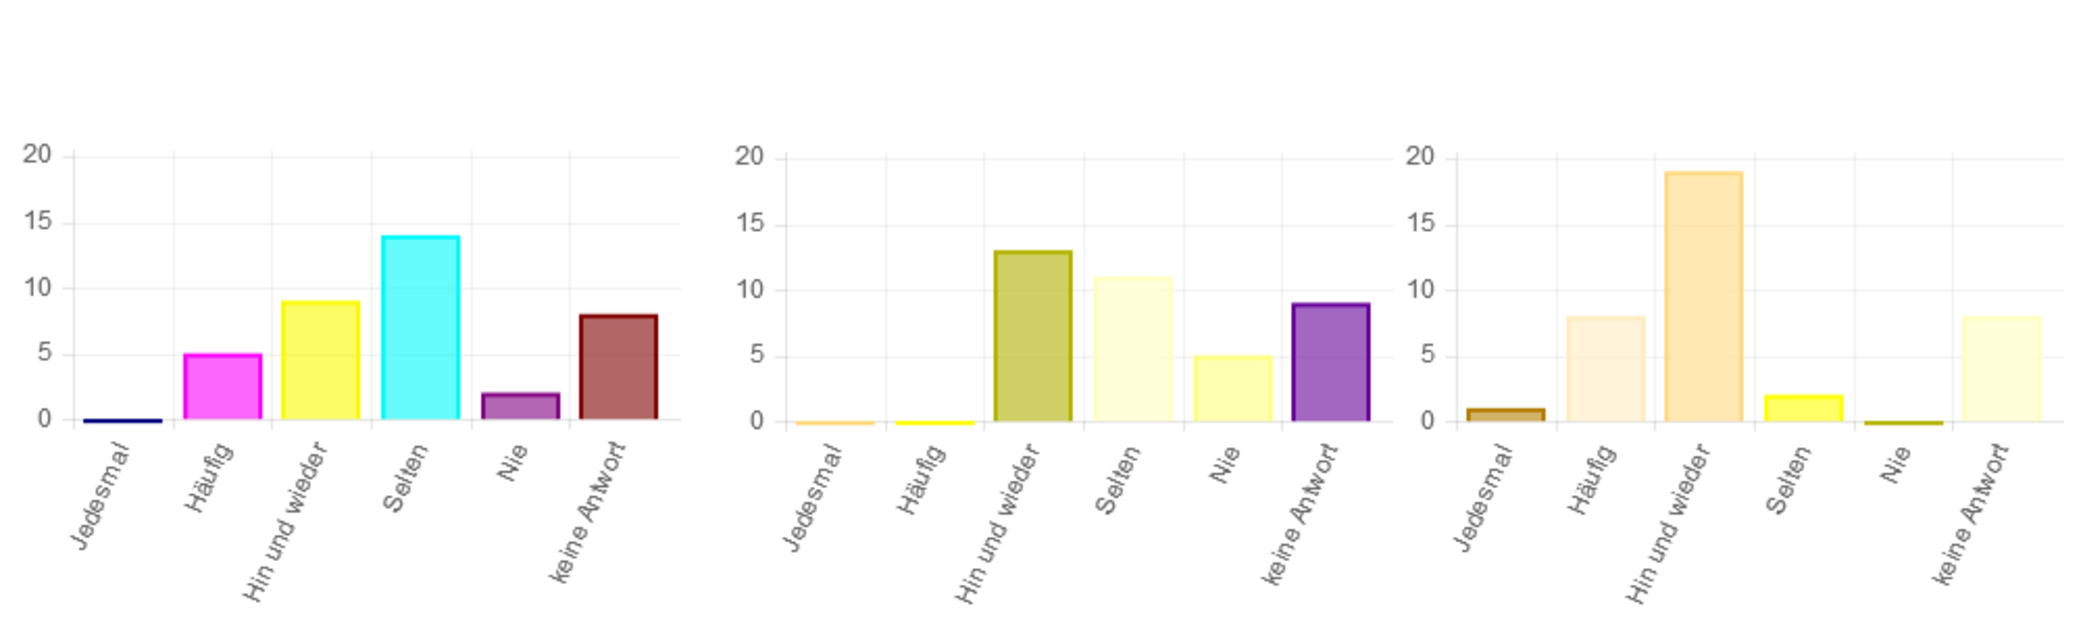
\includegraphics[width=\textwidth, height=\textheight, keepaspectratio]
    {resources/survey-vcs-merge.pdf}
  \caption{Auswertung der Auftrittswahrscheinlichkeit von Merge-Konflikten}
\end{figure}

Die Auswertung der Angaben zu Merge-Konflikten zeigt einen Trend zu einem regelmäßigem Auftreten von Merge-Konflikten. Mit einer Wahrscheinlichkeit von 53\% treten sowohl bei Pull-, als auch bei Push- und Merge-Operationen Merge-Konflikte auf. Dieser Wert ist für den Merge von Branches am höchsten mit 82\%. 

\subsection{Verwendung von Tests}

\begin{figure}[htbp]
  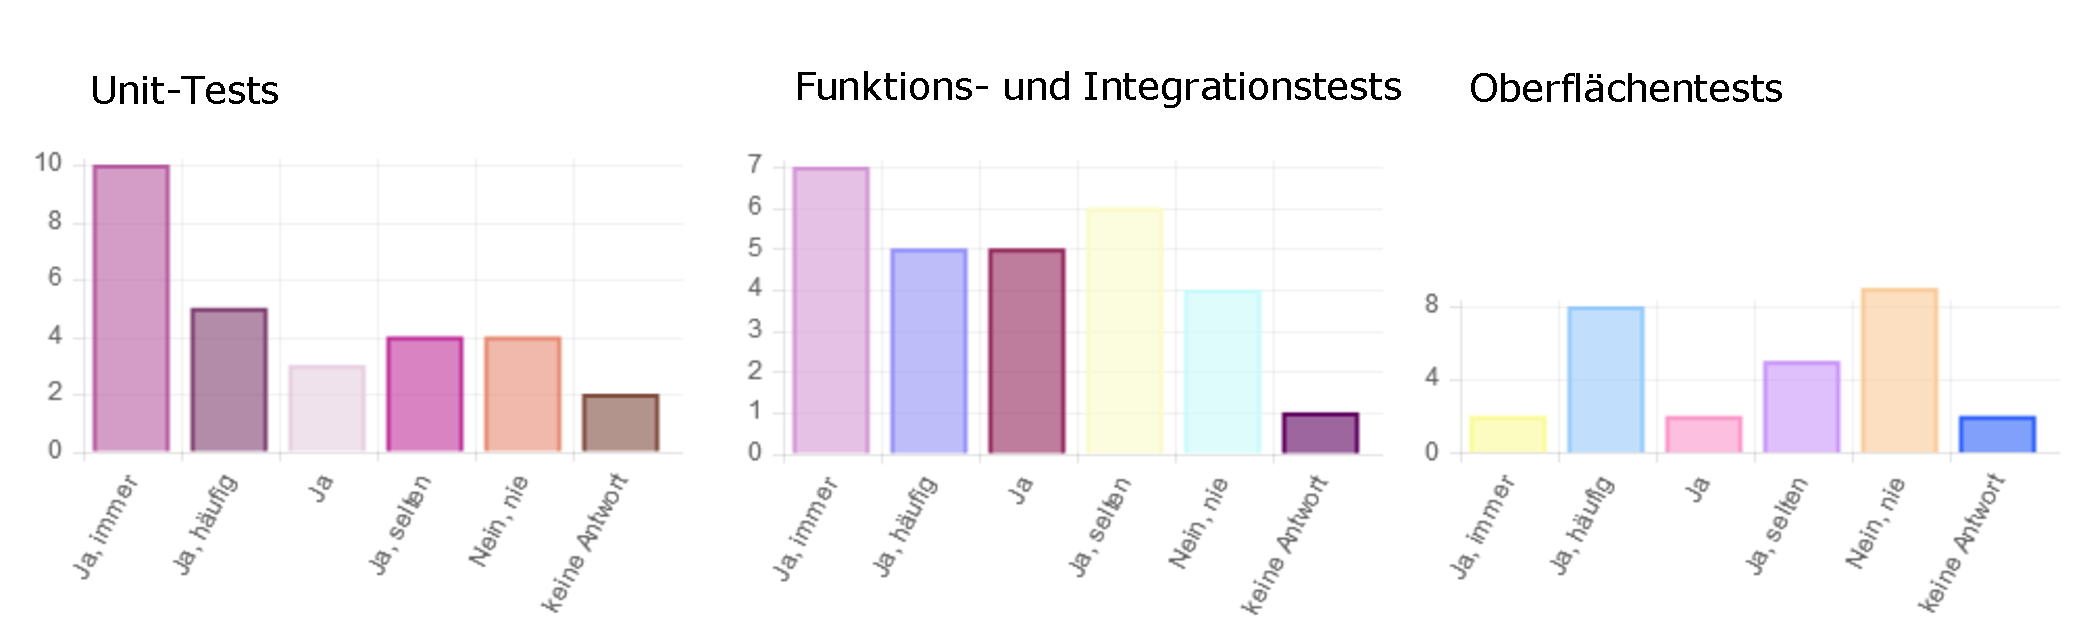
\includegraphics[width=\textwidth, height=\textheight, keepaspectratio]
    {resources/survey-test-usage.pdf}
  \caption{Auswertung der Nutzung von Unit-, Funktions- und Oberfächentests}
\end{figure}

Test werden vom Großteil der Teilnehmer verwendet. Insbesondere Unit-(72\%), Funktions- und Integrationstests(68\%) wurden mit einer hohen Nutzung angegeben. Sichtbar weniger wurden Oberflächentests mit 48\% verwendet.

\paragraph{Weiterführende Tests}

\begin{figure}[htbp]
  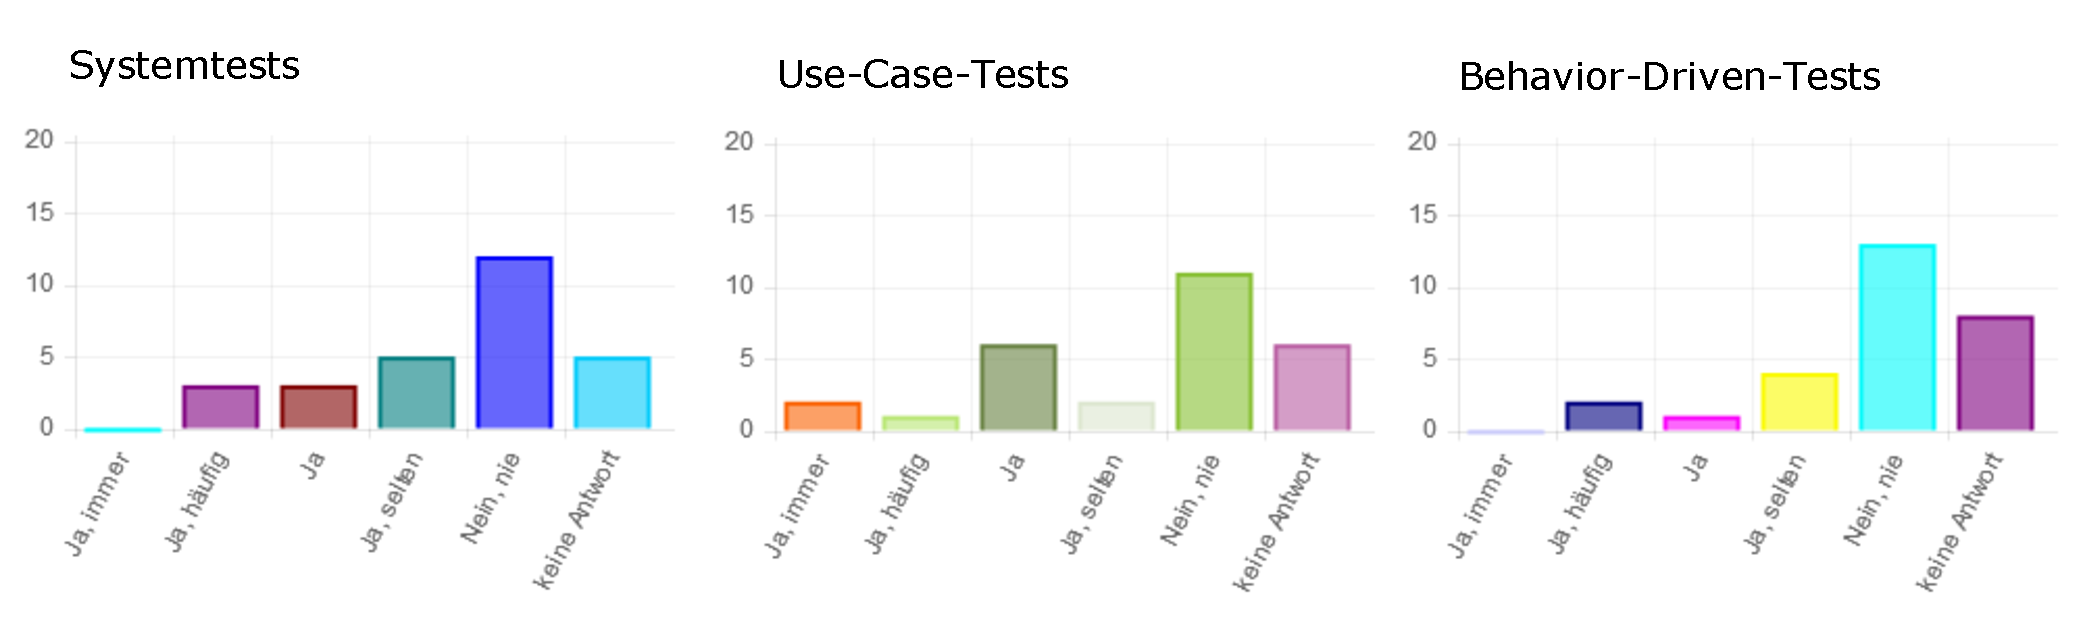
\includegraphics[width=\textwidth, height=\textheight, keepaspectratio]
    {resources/survey-test-usage-special.pdf}
  \caption{Auswertung der Nutzung von System-, Use-Case- und Behavior-Driven-Tests}
\end{figure}

Werden die Angaben zu weiterführenden Testvarianten betrachtet, fallen die deutlich niedrigeren Nutzungsangaben auf. Durchweg wurden Systemtests(24\%), Use-Case-Tests(36\%) und Behavior-Driven-Tests(12\%) deutlich geringer gewählt. Insbesondere bei der Zusammensetzung der Zustimmung wird dies deutlich. Während bei Unit- und Funktionalen-Tests mit 54\% \glqq immer\grqq{} und \glqq häufig\grqq{} gewählt wurden, beliefen sich die Angaben für System-, Use-Case- und Behavior-Driven-Tests nur auf 11\%.

Bezogen auf die Gruppe der Softwareentwickler ist hervorzuheben, dass 10\% der Entwickler weder Unit- noch Funktionstests durchführen. Für die weiterführende Test liegt die Gruppe der Softwareentwickler, die diese nicht verwenden zwischen 30\% und 40\%.

\paragraph{Nutzung von Metriken}

\begin{figure}[htbp]
  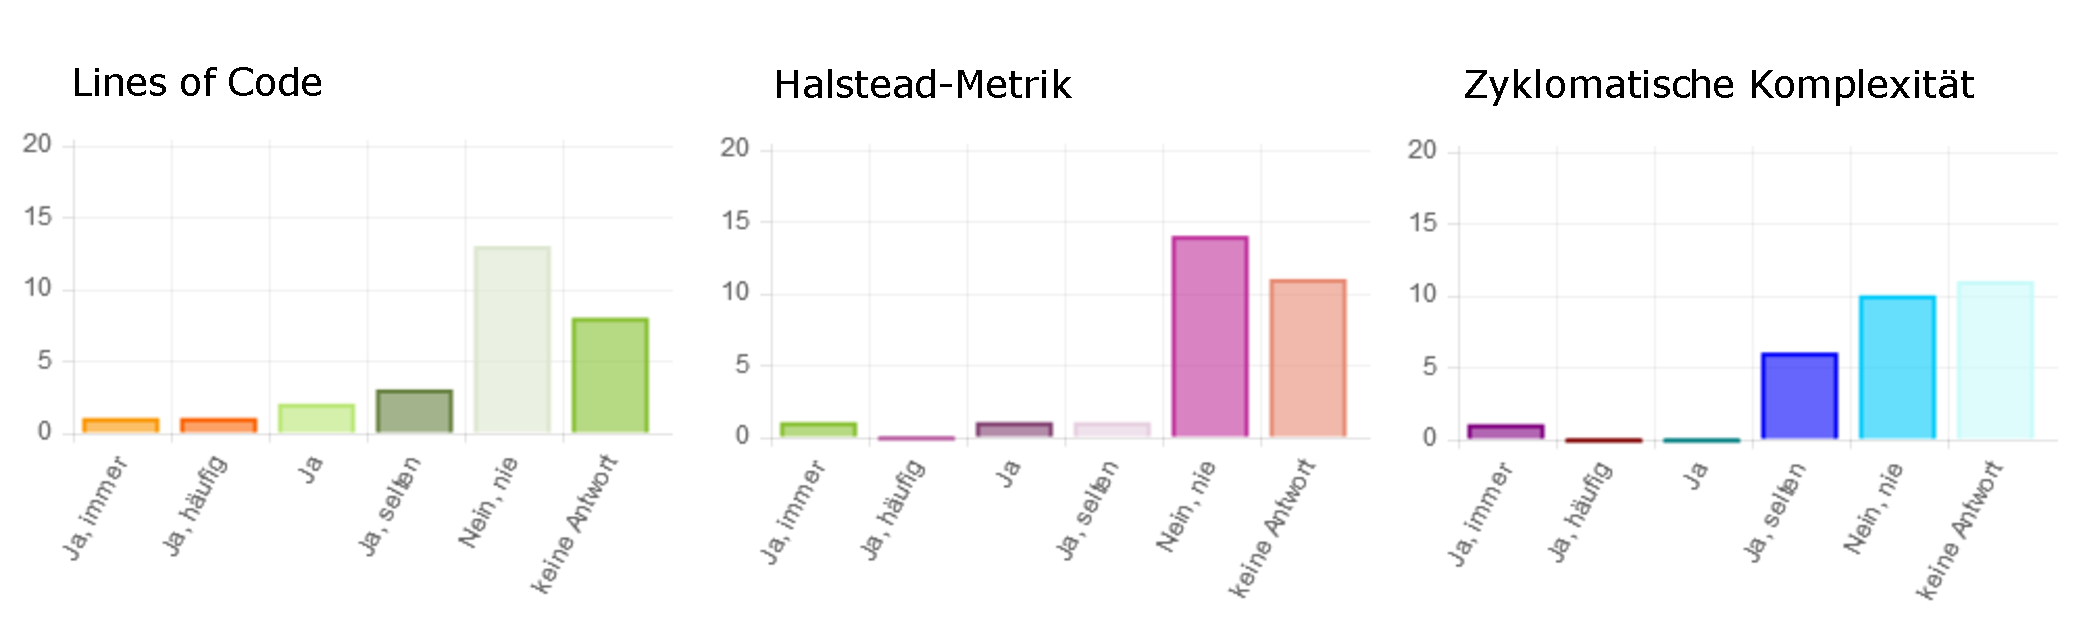
\includegraphics[width=\textwidth, height=\textheight, keepaspectratio]
    {resources/survey-test-usage-metric.pdf}
  \caption{Auswertung der Metrik-Nutzung von Lines-Of-Code, Halstead, und McCabe(Zyklomatische Komplexität)}
\end{figure}

Im Vergleich zur Test-Nutzung werden Metriken deutlich weniger verwendet. Lines-Of-Code wurden mit angegebenen 20\% auf häufigsten Verwendet. Die Komplexitätsmetriken Halstead und McCabe wurden im Schnitt nur von 6\% der Teilnehmer verwendet. Wird die Gruppe auf die teilnehmenden Softwareentwickler beschränkt steigt dieser Wert auf ca. 10\%.

Ergänzend gaben 88\% der Teilnehmer mit dem Begriff der Metrik vertraut zu sein und 80\% der Teilnehmer würde gerne mehr Metriken nutzen oder damit anfangen.

\subsection{Bewertung der Umfrage}

Aufgrund der nicht repräsentativen Teilnehmermenge ist es nicht möglich eine generelle Aussage zu treffen. Die Bewertung ist daher nur begrenzt verwendbar.

Die Angaben des Teilnehmerfelds deuten auf gute Verwendung von Versionsverwaltungssystemen, sowie Unit- und Funktionstests. Bei den betrachteten weiterführenden Techniken ergeben sich durchweg geringere Verwendungen.

Die Studie lässt keine Rückschlüsse zu warum die Verwendung gering ausfällt. Die Verwendung von Feature-Branches könnte durch eine durchgängige Verwendung von Continuous-Integration begründet sein. Die Mangelnde Verwendung von weiterführenden Tests und Metriken ist ohne weitere Studien nicht zu ermitteln.

\section{Prototyp zur Feature-Branch-Visualisierung}

Mit wachsender Beliebtheit von Feature-Branches, erweiterten auch die Anbieter für Continuous-Integration-Lösungen ihr Angebot. Viele Anbieter stellen umfangreiche Angebote für Continuous-Deployment bereit. Oftmals sind auch zusätzliche Optionen für Feature-Branches enthalten. Wie im Git-Workflow vorgestellt, werden diese Feature-Branches durch einen manuellen Merge-Befehl auf einem Release-Branch akkumuliert. Auf diese Weise werden kontinuierlich, wenn auch verzögert, die einzelnen Feature-Branches mit einander zusammengeführt. Das späte Feedback zum Zeitpunkt der Zusammenführung, kann zu Problemen und zur Verzögerungen beim Release führen. Eine direkte Alternative ist es, die jeweiligen Feature-Branches direkt zum Zeitpunkt ihrer Fertigstellung zusammenzuführen. Für jeden weiteren Feature-Branch, der zusammengeführt werden muss, ergeben sich allerdings die gleichen Problem, wie bereits zuvor.
Eine mögliche Lösung wäre es Release bereits im Vorfeld zu definieren und die dazugehörigen Branches zu verfolgen. Somit können Konflikten in Codeständen und potentielle Fehlerquellen eher erkennen. Sind alle Feature-Branches konfliktfrei, können diese automatisch zu einem Release gebündelt werden. Jeder einzelne Branch kann durch Tests und Metriken unterstützt werden. Zudem können auf diese Weise Features zurückgehalten werden, die fertig gestellt wurden, aber aus politischen Gründen noch nicht Teil des Releases sein dürfen. 
Die Behebung von Merge-Konflikten bedeutet, dass einer der beiden vom Konflikt betroffenen Branches, Teile des Codes des anderen Branches, mit aufnehmen muss. Daher ist es möglich, dass auch mit der Verwendung von Feature-Branches, das gezielte zurückhalten von Features, schwierig bleibt. Daher können dieses beiden Branches nicht ohne ein Feature-Toggle unabhängig von einander veröffentlicht werden.

Der Prototyp soll somit die folgenden Punkte unterstützen:
\begin{itemize}
\item Gruppierung von Feature-Branches zu Releases,
\item Darstellung der Untermenge an Branches, welche bereits zu einem Release kombiniert werden können,
\item Darstellung der Testergebnisse, Testabdeckung und Code-Qualitätsmetriken und
\item Bereitstellung einer API um Testergebnisse und Metriken mit einem Continuous-Integration-System zu synchronisieren.
\end{itemize}

\subsection{Anforderungen}

Ziel des Prototyps ist es Release-Informationen zu einem Projekt anzuzeigen. Daher müssen Projekte angelegt und bearbeitet werden. Zudem müssen die zugehörigen Repository-Informationen ausgelesen werden. Weiter sollten Abhängigkeiten des Projektes ausgelesen und ausgewertet werden. 

Um einzuordnen, welche Änderungen zu einem Release gehören, müssen diese Änderungen definiert werden. Im Fall von Feature-Branches müssen die Feature-Branches deklariert werden, welche Teil des Releases werden. Damit ein Release aussagekräftig deklariert wird, sollten zudem Feature-Branches innerhalb der Abhängigkeiten deklariert werden.

Ist das Release definiert, sollen eine Reihe an Fragen einfach zu beantworten sein. 
\begin{itemize}
\item Können alle Feature-Branches zusammengeführt werden?
\item Welche Branches würde einen Konflikt mit welchem anderen Branch auslösen?
\item Wie sieht die derzeit minimal release-fähige Untermenge an Feature-Branches aus?
\item Welche Branches wurden erfolgreich getestet?
\item Wie verhalten sich die Metriken der Feature-Branches untereinander und zum Haupt-Branch?
\end{itemize}

Des Weiteren sollte die Anbindung an einen bestehenden Continuous-Prozess möglich sein. Es sollte daher eine REST-API bereit gestellt werden. Die API soll primär die Daten für Metriken und Testergebnisse entgegennehmen.

\subsection{Nutzungsszenarien (Use-Cases)}

Aus den Anforderungen ergeben sich einige Nutzungsszenarien. Es soll keine vollständige Projektspezifikation für den Prototypen erstellt werden, daher werden die Nutzungsszenarien nur angerissen. 

\paragraph{Projekt registrieren}
Um die Projekte zu analysieren, müssen sie angelegt werden. Im optimal Fall geschieht dies durch die Angabe eines Repositories. Aus diesem Repository können, anhand der Beschreibungsdatei der verwendeten Packetverwaltung, die weiteren Informationen gewonnen werden.

\paragraph{Branches auflisten}
Um die Feature-Branches für ein Release zu selektieren, müssen alle verfügbaren Branches des Projektes dargestellt werden. 

\paragraph{Release erstellen}
Die Release-Erstellung erfolgt durch die Wahl eines Namens und der Selektion der gewünschten Branches. Der Release wird dem Projekt zugeordnet und kann über das Projekt angezeigt werden.

\paragraph{Branch-Details darstellen}
Um einen Branch zu bewerten, müssen Tests und Metriken für den Branch ausgeführt werden. Die Ausführung und die Sammlung der Daten werden außerhalb des Tools durchgeführt, daher werden diese Daten über eine API zugeführt.

\paragraph{Branch-Konflikte anzeigen}
Zur weiteren Bewertung der Branches müssen Merge-Konflikte zwischen den Branches ermittelt werden. Branches, die einen Konflikt aufweisen, sollten in der Release-Übersicht markiert und gruppiert werden.

\paragraph{Release abschließen}
Um ein Release abzuschließen, müssen alle Feature-Branches ohne Konflikt zusammengefasst werden. Dafür muss ein eigener Release-Branch erstellt werden. Auf den Release-Branch werden alle Feature-Branches durch einen Fast-Forward-Merge zusammengefasst. Abschließend wird das Release mit einem Tag versehen. Der Tag kann zum Vorgänger Tag um eine eine Major\hyp{}, Minor\hyp{} oder Patch\hyp{}Versionsnummer ansteigen.

\subsection{Grundlagen der Umsetzung}

Da der Prototyp als Unterstützung für bestehende Werkzeuge agieren soll, bietet sich ein modernes Web-Framework an. Durch die berufliche Prägung des Autors der Masterarbeit, liegt der Fokus zudem auf PHP. Die Wahl für ein modernes und flexibles Framework fällt daher auf Symfony, welches sich durch Flexibilität und Modularität auszeichnet. Zudem existiert für Symfony eine sehr aktive Community, welche Zahlreiche Werkzeug und Hilfsbibliotheken bereit stellt. Durch Symfony ergibt sich als bevorzugte Abhängigkeitsverwaltung Composer.  

\subsection{Domainmodell}

Das betrachtete Problem betrifft sowohl Repository-Artefakte, als auch Projekt- und Release-Details. Weiter müssen Metriken und Testergebnisse protokolliert werden. Da die Erstellung von Metriken und Tests eine größere Zeitspanne benötigen kann, sollten die Ergebnisse persistiert werden. 

\begin{figure}[htbp]
  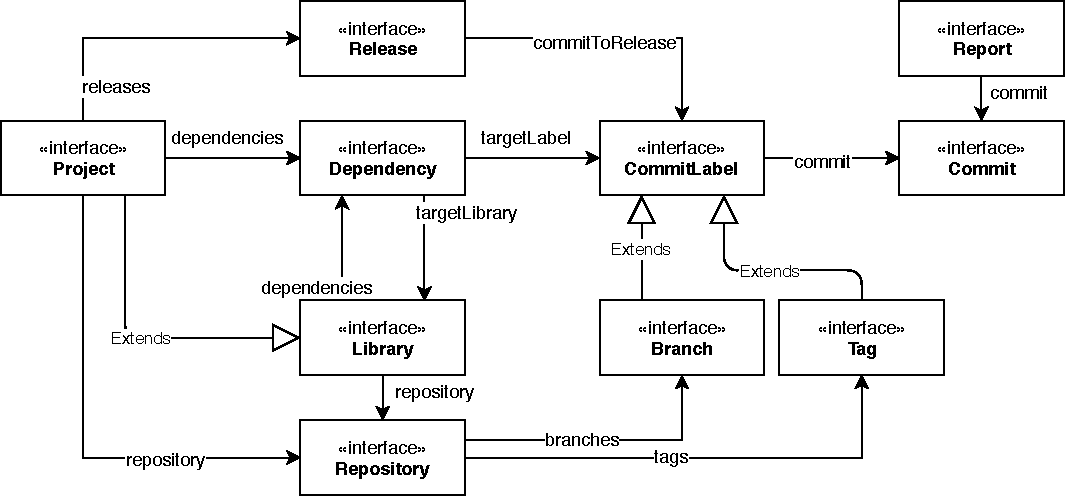
\includegraphics[
    width=\textwidth,
    height=\textheight,
    keepaspectratio
  ]{resources/ReleaseWardenClassChart.pdf}
  \caption{Klassendiagramm für Domainmodell}
  \label{class-chart-release-warden}
\end{figure}

In Abbildung~\ref{class-chart-release-warden} wird das Domainmodell in einem UML-Klassendiagramm dargestellt. Das Domainmodell beschreibt ein betrachtetes Projekt(Project) mit seinen Abhängigkeiten(Dependency) und den Releases für das Projekt. 
Um die Abhängigkeiten abzubilden und die verfügbaren Feature-Branches für ein Release zu selektieren, werden somit auch die Repositories und ihre Branches und Tags benötigt.

\subsection{Umsetzung der Nutzerszenarien}

\paragraph{Projekt registrieren}

\paragraph{Branches auflisten}

\paragraph{Release erstellen}

\paragraph{Branch-Details anzeigen}

\paragraph{Branch-Konflikte anzeigen}

\paragraph{Release erstellen}

Beschreibung von PHPMetrics

\section{Motivation, Disziplin und Verantwortung - Faktor Mensch}
\label{sec:human-fail}
Die vorangegangene Kapitel beschäftigen sich größtenteils mit Methodiken und Hilfsmitteln. Die Motivation dieser Methodiken und Hilfsmittel begrenzt sich unter anderem auf Wartbarkeit, Robustheit und Skalierbarkeit von Software. Dabei wird die Motivation für die Entwicklung, genauer für den Entwickler, weitestgehend ausgelassen.

Gerade in Anbetracht der Zeit, die viele der Methodiken bereits bekannt sind, ist es hilfreich einen weiteren Aspekt hinzuziehen. Dieser Aspekt soll den psychischen Teil der Einführung einer neuen Methodik beleuchten.

\subsection{Motivation}

Motivation kann durch drei Bereiche getragen werden\footcite[vgl.][]{codingame-drive}\footcite[vgl.][Kap. Autonomie ff.]{pink-drive}:
\begin{itemize}
\item Autonomie - die Möglichkeit sich selbst zu organisieren. Autonomie soll die eigenen Fähigkeiten möglichst voll nutzen.
\item Können - die Möglichkeit sich weiterzuentwickeln und Neues zu entdecken.
\item Bestimmung - die Möglichkeit an etwas mit Bedeutung mitzuwirken.
\end{itemize}

Die Einteilung ist eine Zusammenfassung mehrere einzelner Theorien und in manchen Teilen populärwissenschaftlich\footcite[vgl.][]{drive-scholarly-review}. 

Basierend auf den drei Bereichen, können die Methodiken besser argumentiert und die generelle Bereitschaft zur Einführung gestärkt werden. Generell sollte jeder Teilnehmer einer Methodik sich darin wiederfinden. Methodiken die sich nicht im Alltag des Entwicklungsteams wiederfinden, werden auf lange Sicht verschwinden oder zur Belastung.

\subsection{Disziplin}

Viele eingeführte Hilfsmittel, Methodiken oder Ideen verschwinden wieder. Oftmals fehlen Träger und Fürsprecher. Häufig fehlt es aber auch an Disziplin. Entscheidend ist die Einsicht zur Selbstdisziplin. Viele agile Methodiken basieren auf Selbstorganisation und Eigenverantwortung\footcite[vgl.][]{codingame-agile-failed}. Die Methodiken setzen einen Entwickler voraus, der bereit ist stetig zu wachsen und an sich zu arbeiten.
Disziplin greift nach der Motivation. Nach der Einführung einer neuen Methodik, benötigt es oft Disziplin diese aktiv zu nutzen\footcite[vgl.][]{screw-motivation}. Es benötigt konstante Arbeit und Reflexion zur Nutzung und Erhaltung einer neuen Methodik.

Oftmals ist eine neue Methodik damit verbunden, alte Verhaltensweisen abzulegen.
Gelernte Verhaltensweise lassen sich oft eine Folge von drei Punkten gliedern.
\begin{itemize}
\item Auslöser - die Situation, welche eine Gewohnheit auslöst oder diese einleitet.
\item Verhalten - der Ablauf oder das Verhalten, welches die Gewohnheit darstellt.
\item Nutzen - der Nutzen, welchen das Verhalten erzeugt.
\end{itemize}
Die Hemmschwelle zur Einführung einer neuen Methodik sollte möglichst gering gehalten werden. Dazu bietet es sich an die Methodik an bereits existierende Mechanismen zu knüpfen. Zudem sollte der Aufwand die Methodik zu nutzen sehr gering und der Nutzen durch eine Rückkopplung spürbar sein\footcite[vgl.][]{steps-of-habit}.

\subsection{Verantwortung}

Auch eine Methodik die durch Träger und Fürsprecher eingeführt wird, sollte in der Verantwortung des ganzen Entwicklungsteam liegen. Die Einhaltung der Methodik sollte jeden in die Verantwortung ziehen. Wird die Methodik missachtet sollte ein direktes Feedback darauf hinweisen. Dieser Hinweis sollte auf keinen Fall öffentlich oder anklagend sein. Ebenso sollte jegliche Form der Bestrafung ausgeschlossen werden.

Wie auch in vielen agilen Methodiken, ist eine gemeinsame Fürsprache, ein gemeinsames \glqq \gls{Commitment}\grqq{} notwendig. Ein gemeinsames Commitment sollte, wenn möglich, durch technische Hilfsmittel unterstütze werden. Für viele gemeinsame Regeln existieren automatisierte Prüfungen oder Integrationen für die Entwicklungsumgebung und den automatisierten Software-Erstellungsprozess.
Auch der Review-Prozess für Softwareänderungen kann hierbei unterstützen. Entwickler sollten sich stets gegenseitig auf die Missachtung von Coding-Guidelines und Entwicklungsmustern hinweisen.

\subsection{Faktor Mensch}

Die Erstellung von Software verlangt eine breite Palette an Fähigkeiten. Zudem fehlen in der Softwareerstellung viele der standardisierten Vorgehensweisen der Ingenieursdisziplinen. Häufig werden kreative und pragmatische Lösungen benötigt.

\blockquote {discipline, the most lacking virtue in creative people (like programmers)}\footcite[][S.167]{git-essentials-2017}
\vspace{1em}\\
Die fehlenden Standards und Notwendigkeit für kreativen Lösungen von Entwicklern, sind ein zu respektierendes Risiko in der Softwareentwicklung. Fordernde und anspruchsvolle Methodiken sind nicht für alle Softwareentwickler geeignet. Laufende Projekte und bestehende Belastungen sind bei der Einführung neuer Methodiken stets zu beachten. Die Einführung neuer Methodiken in bereits belastete oder scheiternde Projekte führen oft zu schlimmeren Ergebnissen.

Neue Methodiken sollten stets mit dem nötigen Raum eingeführt werden. Zudem sollte eine regelmäßige Betrachtung des Verhältnisses von Aufwand und Nutzen erfolgen.
